\documentclass[12pt,a4paper]{article}
\usepackage[utf8]{inputenc}
\usepackage[T1]{fontenc}
\usepackage[brazil]{babel}
\usepackage{lmodern}
\usepackage[margin=2.5cm]{geometry}
\usepackage{graphicx}
\usepackage{booktabs}
\usepackage{amsmath,amssymb}
\usepackage{float}
\usepackage{caption}
\usepackage{array}
\usepackage{microtype}
\usepackage[dvipsnames]{xcolor}
\usepackage[colorlinks=true,linkcolor=blue!50!black,urlcolor=blue!50!black,citecolor=blue!50!black]{hyperref}
\graphicspath{{../figuras/}}
\captionsetup{font=small,labelfont=bf}
\setlength{\parskip}{0.5em}
\setlength{\parindent}{0pt}

\newcommand{\dgpa}{\ensuremath{\Delta\mathrm{GPA}}}

\title{\textbf{Impacto do uso passivo vs.\ ativo de IA\\generativa no \dgpa{}:\\Experimento fatorial $2^3 r$\\com bootstrap estratificado}\\[0.3em]
\large Relat\'orio da Entrega 2 -- Resultados preliminares}
\author{Wagner Tironi Pinto\\[0.2em]
\small Orientador: Prof.\ Dr.\ Carlos H.\ G.\ Ferreira\\
\small PCC170 -- Projeto e An\'alise de Experimentos Computacionais}
\date{}

\begin{document}
\maketitle

\begin{abstract}
Este relat\'orio apresenta a Entrega 2 do projeto de PCC170. Avalia-se se o modo de uso de IA generativa
(\emph{passivo}: gerar texto/resposta pronta; \emph{ativo}: idear, resumir, depurar) afeta a varia\c{c}\~ao
de desempenho acad\^emico (\dgpa{} $=$ GPA p\'os $-$ GPA pr\'e), em interação com a ansiedade em exames e as horas de estudo.
O recorte \'e \'unico (STEM + \emph{Junior}, $n=3.279$) e os n\'iveis dos fatores s\~ao definidos pela mediana ($Q_2$):
\emph{baixo} $\le Q_2$ e \emph{alto} $>Q_2$, o que aproveita todos os alunos do recorte (menor c\'elula com 181 alunos).
Utiliza-se um projeto fatorial $2^3$ com $r=30$ r\'eplicas
obtidas por bootstrap estratificado (semente 42, $m=36$ alunos por c\'elula), e um segundo ciclo de bootstrap (5.000 reamostras)
para intervalos de confian\c{c}a dos efeitos. O efeito das horas de estudo \'e dominante ($+0{,}121$; 61,7\% da vari\^ancia);
o uso passivo reduz o \dgpa{} em $0{,}077$ (IC95\% $[-0{,}092;-0{,}062]$) e interage negativamente com a ansiedade
($-0{,}023$). A regra por quartis extremos ($<Q_1$/$\ge Q_3$) \'e mantida como an\'alise de sensibilidade e leva \`as mesmas conclus\~oes qualitativas.
Os resultados s\~ao preliminares e observacionais, e as limita\c{c}\~oes s\~ao discutidas.
\end{abstract}

\tableofcontents
\newpage

%=====================================================================
\section{Introdu\c{c}\~ao}
%=====================================================================
\textbf{Contexto.} A ado\c{c}\~ao de IA generativa por estudantes universit\'arios cresceu rapidamente, mas h\'a
d\'uvida sobre se seus benef\'icios dependem da \emph{forma} de uso. Usos que substituem o esfor\c{c}o cognitivo
(obter respostas prontas, redigir textos) tendem a ser distintos de usos que o ampliam (gerar ideias, resumir leituras, depurar c\'odigo).

\textbf{Motiva\c{c}\~ao e problema.} Na Entrega 1 foi estimado, por \emph{propensity score matching}, um efeito m\'edio
do uso passivo de $\text{ATE}=-0{,}072$ (IC95\% $[-0{,}092;-0{,}053]$). Ap\'os orienta\c{c}\~ao do professor, o problema foi
reformulado: (i) adotar um \'unico recorte (STEM + \emph{Junior}) para evitar vi\'es de composi\c{c}\~ao; (ii) usar
bootstrap e um projeto fatorial para normalizar os dados e quantificar efeitos e intera\c{c}\~oes.

\textbf{Objetivo.} Quantificar o efeito do modo de uso da IA (A), da ansiedade em exames (B) e das horas de estudo
tradicionais (C), e suas intera\c{c}\~oes, sobre o \dgpa{}.

\textbf{Hip\'otese geral (definida antes do experimento).} $H_0$: nenhum dos efeitos principais ou de intera\c{c}\~ao
sobre o \dgpa{} \'e diferente de zero. $H_1$: o uso passivo reduz o \dgpa{} em relação ao uso ativo, e esse efeito
depende (interage) do n\'ivel de ansiedade e/ou das horas de estudo.

%=====================================================================
\section{An\'alise Explorat\'oria dos Dados}
%=====================================================================
Esta se\c{c}\~ao apenas caracteriza os dados; a avalia\c{c}\~ao da hip\'otese ocorre nas se\c{c}\~oes seguintes.

\subsection{Base de dados}
A base \texttt{ai\_student\_impact\_dataset.csv} possui 50.000 registros e 16 vari\'aveis, sem valores nulos. Trata-se de dados
tabulares (n\~ao simulados pelo autor) cuja origem exata (provavelmente um conjunto p\'ublico sint\'etico do Kaggle) deve
ser citada na vers\~ao final. Vari\'aveis usadas: \texttt{Primary\_Use\_Case}, \texttt{Anxiety\_Level\_During\_Exams} (1--10),
\texttt{Traditional\_Study\_Hours}, \texttt{Pre\_Semester\_GPA}, \texttt{Post\_Semester\_GPA}, \texttt{Major\_Category} e \texttt{Year\_of\_Study}.
A resposta \'e $\dgpa{}=\text{GPA}_{p\acute{o}s}-\text{GPA}_{pr\acute{e}}$.

\subsection{Recorte e estat\'isticas descritivas}
O recorte STEM + \emph{Junior} cont\'em $n=3.279$ alunos (813 passivos e 2.466 ativos).

\begin{table}[H]
\centering
\caption{Estat\'isticas descritivas (base completa e recorte STEM + \emph{Junior}).}
\begin{tabular}{lcccc}
\toprule
Vari\'avel & \multicolumn{2}{c}{Base completa} & \multicolumn{2}{c}{STEM + Junior}\\
 & M\'edia & DP & M\'edia & DP\\
\midrule
\dgpa{} & 0,20 & 0,19 & 0,24 & 0,19\\
Ansiedade (1--10) & 4,27 & 2,14 & 4,42 & 2,23\\
Horas de estudo & 11,21 & 5,16 & 11,04 & 5,29\\
\bottomrule
\end{tabular}
\end{table}

\subsection{Defini\c{c}\~ao dos n\'iveis pela mediana}
No recorte, as medianas ($Q_2$) s\~ao: ansiedade $Q_2=4$ e horas de estudo $Q_2=10{,}91$.
N\'ivel \emph{baixo} $\le Q_2$ e n\'ivel \emph{alto} $>Q_2$. Todos os 3.279 alunos entram no experimento (nenhuma faixa \'e descartada).
Como a ansiedade \'e discreta, 53,4\% dos alunos t\^em ansiedade $\le Q_2$ (horas: 50,0\%).
A regra anterior ($<Q_1$ baixo, $\ge Q_3$ alto, com $Q_1=3$, $Q_3=6$ para ansiedade e $Q_1=7{,}33$, $Q_3=14{,}475$ para horas) descartava 74\% do recorte
e fica como an\'alise de sensibilidade. As Figuras~\ref{fig:dist} e~\ref{fig:n} mostram as distribui\c{c}\~oes, os pontos de corte e o tamanho das c\'elulas.

\begin{figure}[H]\centering
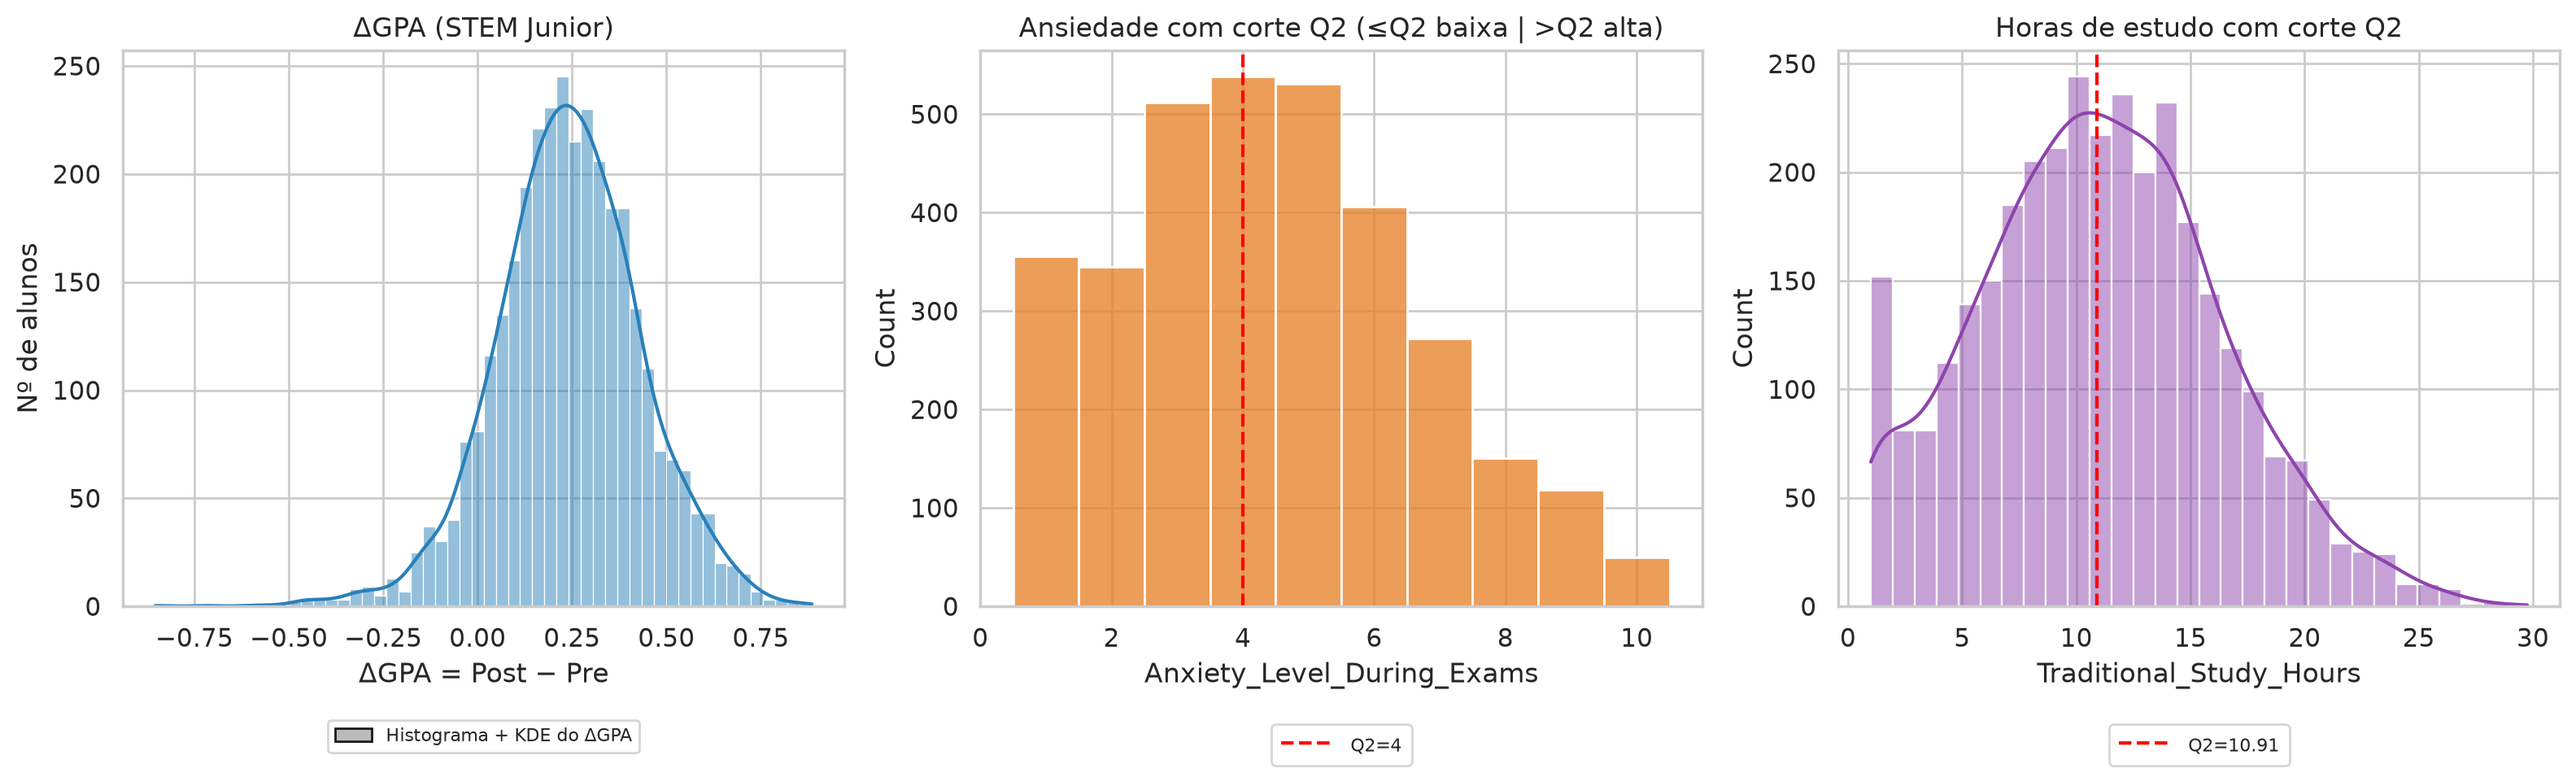
\includegraphics[width=\textwidth]{01_distribuicoes_quartis.png}
\caption{Distribui\c{c}\~oes de ansiedade, horas de estudo e \dgpa{} com o corte pela mediana ($Q_2$).}\label{fig:dist}
\end{figure}

\begin{figure}[H]\centering
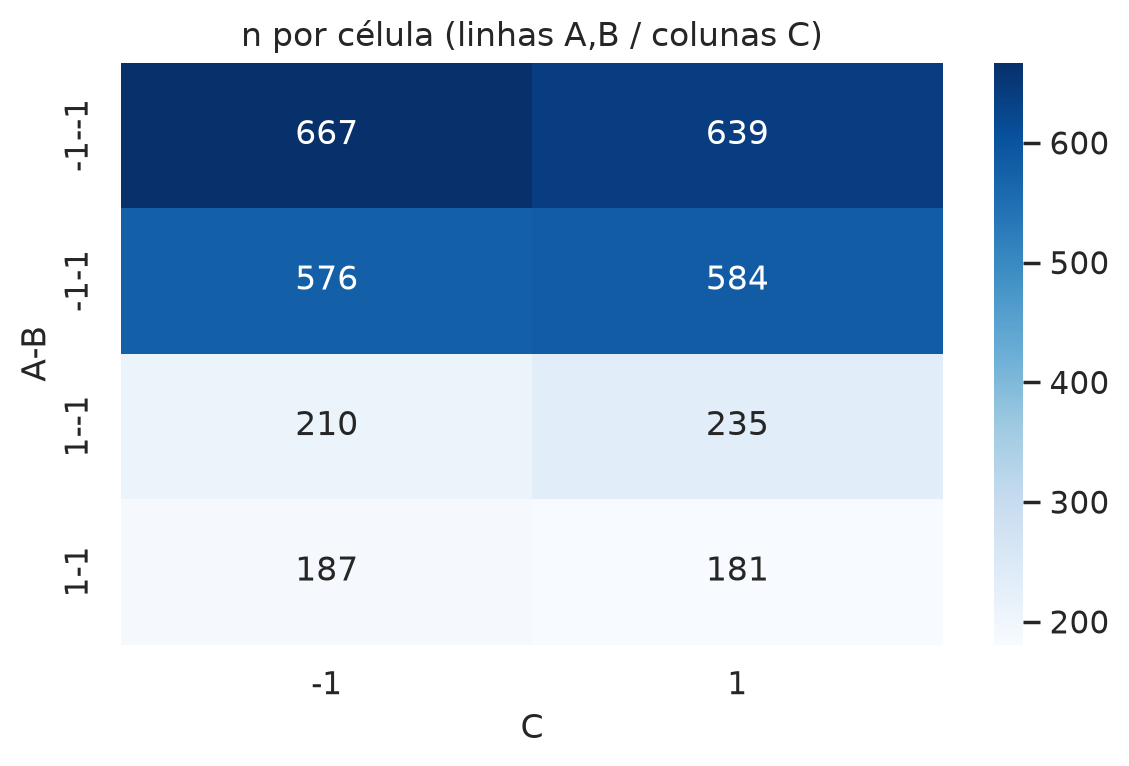
\includegraphics[width=0.8\textwidth]{02_n_por_celula.png}
\caption{N\'umero de alunos por c\'elula do fatorial. A menor c\'elula tem $n=181$ (passivo, ansiedade alta, muito estudo).}\label{fig:n}
\end{figure}

\subsection{Distribui\c{c}\~ao acumulada (CDF)}
As CDFs emp\'iricas permitem comparar os grupos sem depender de agrupamento (\emph{bins}). A Figura~\ref{fig:cdf1}
mostra que a curva do \dgpa{} de usu\'arios passivos est\'a deslocada \`a esquerda, e que a curva de horas altas est\'a deslocada \`a direita (maior \dgpa{}).
A Figura~\ref{fig:cdf2} compara as oito c\'elulas e o recorte completo com o subconjunto de extremos $Q_1/Q_3$ (anal\'ise de sensibilidade).
A Figura~\ref{fig:cdf3} mostra as vari\'aveis cont\'inuas com o corte $Q_2$ (e $Q_1$, $Q_3$ como refer\^encia).

\begin{figure}[H]\centering
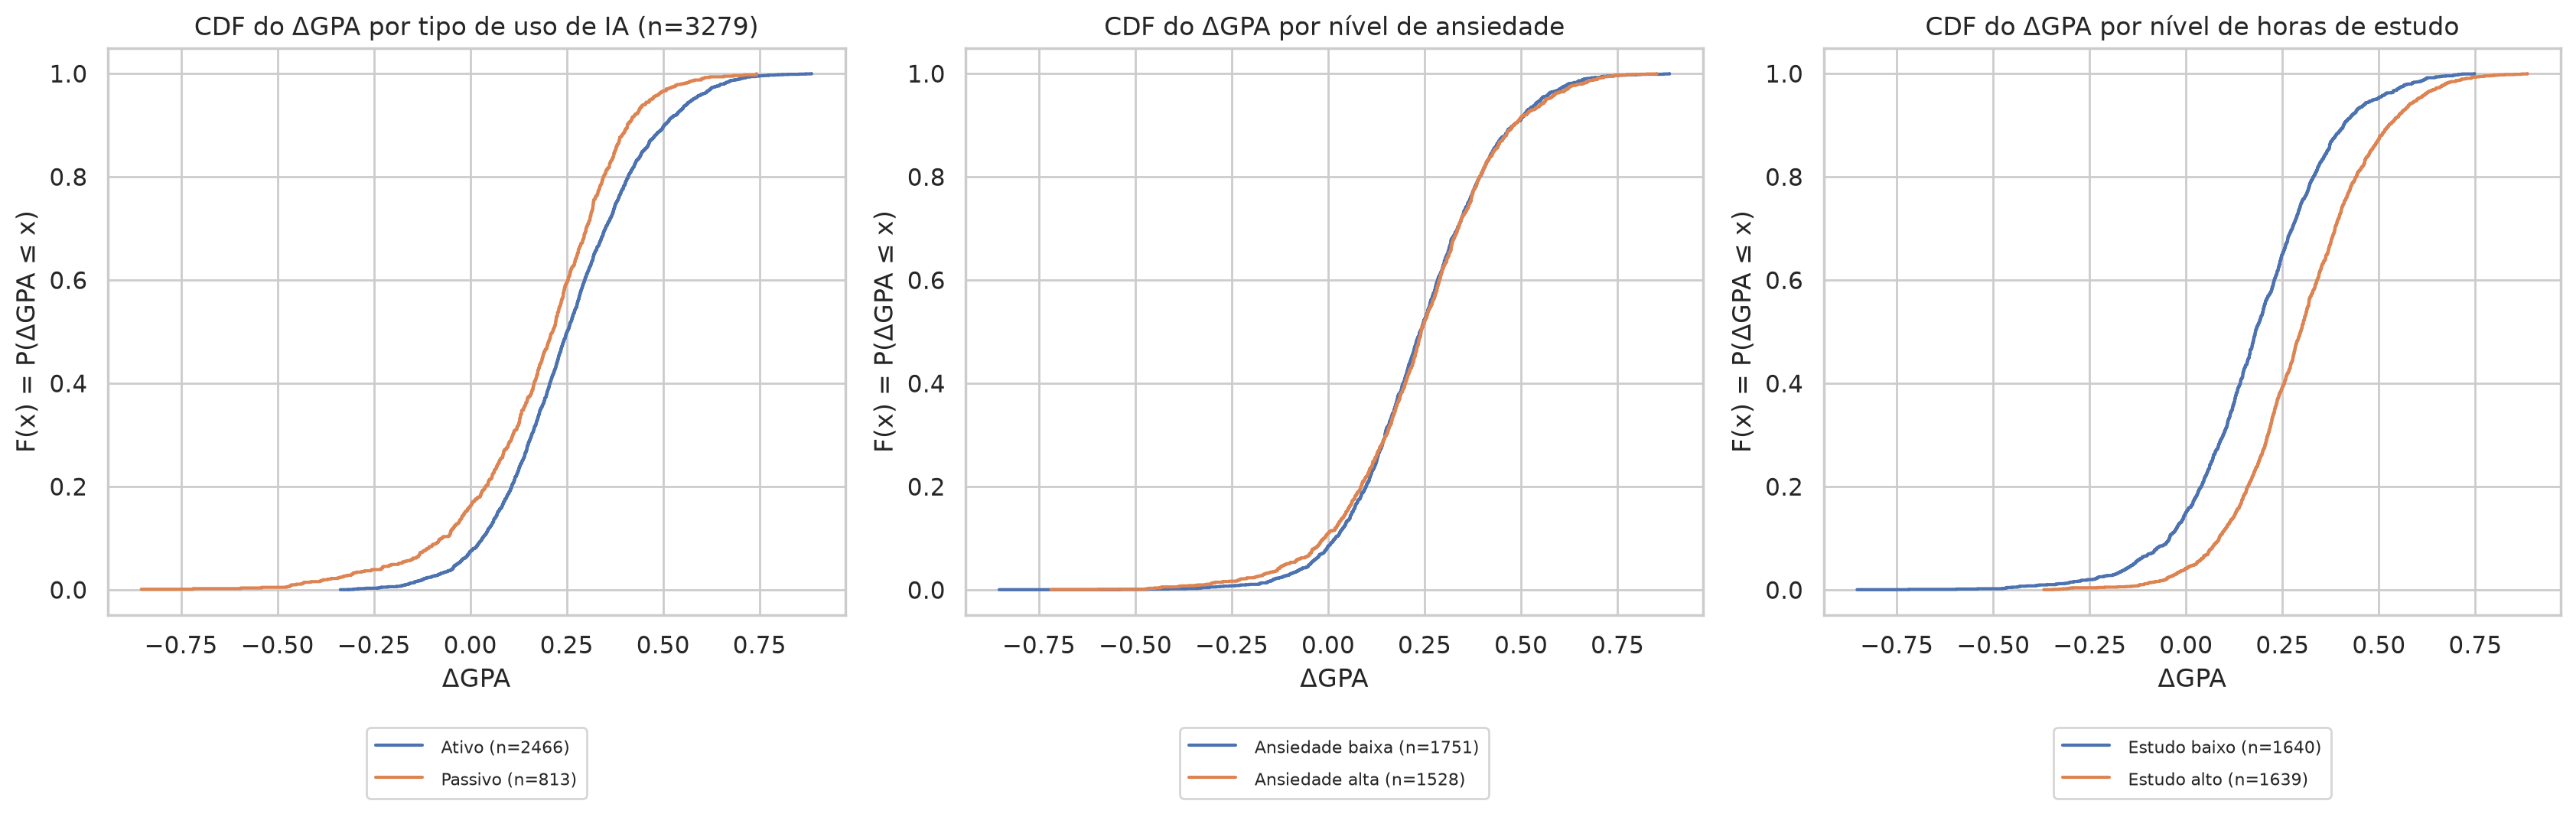
\includegraphics[width=\textwidth]{15_cdf_fatores.png}
\caption{CDF do \dgpa{} segundo cada fator (A, B e C).}\label{fig:cdf1}
\end{figure}

\begin{figure}[H]\centering
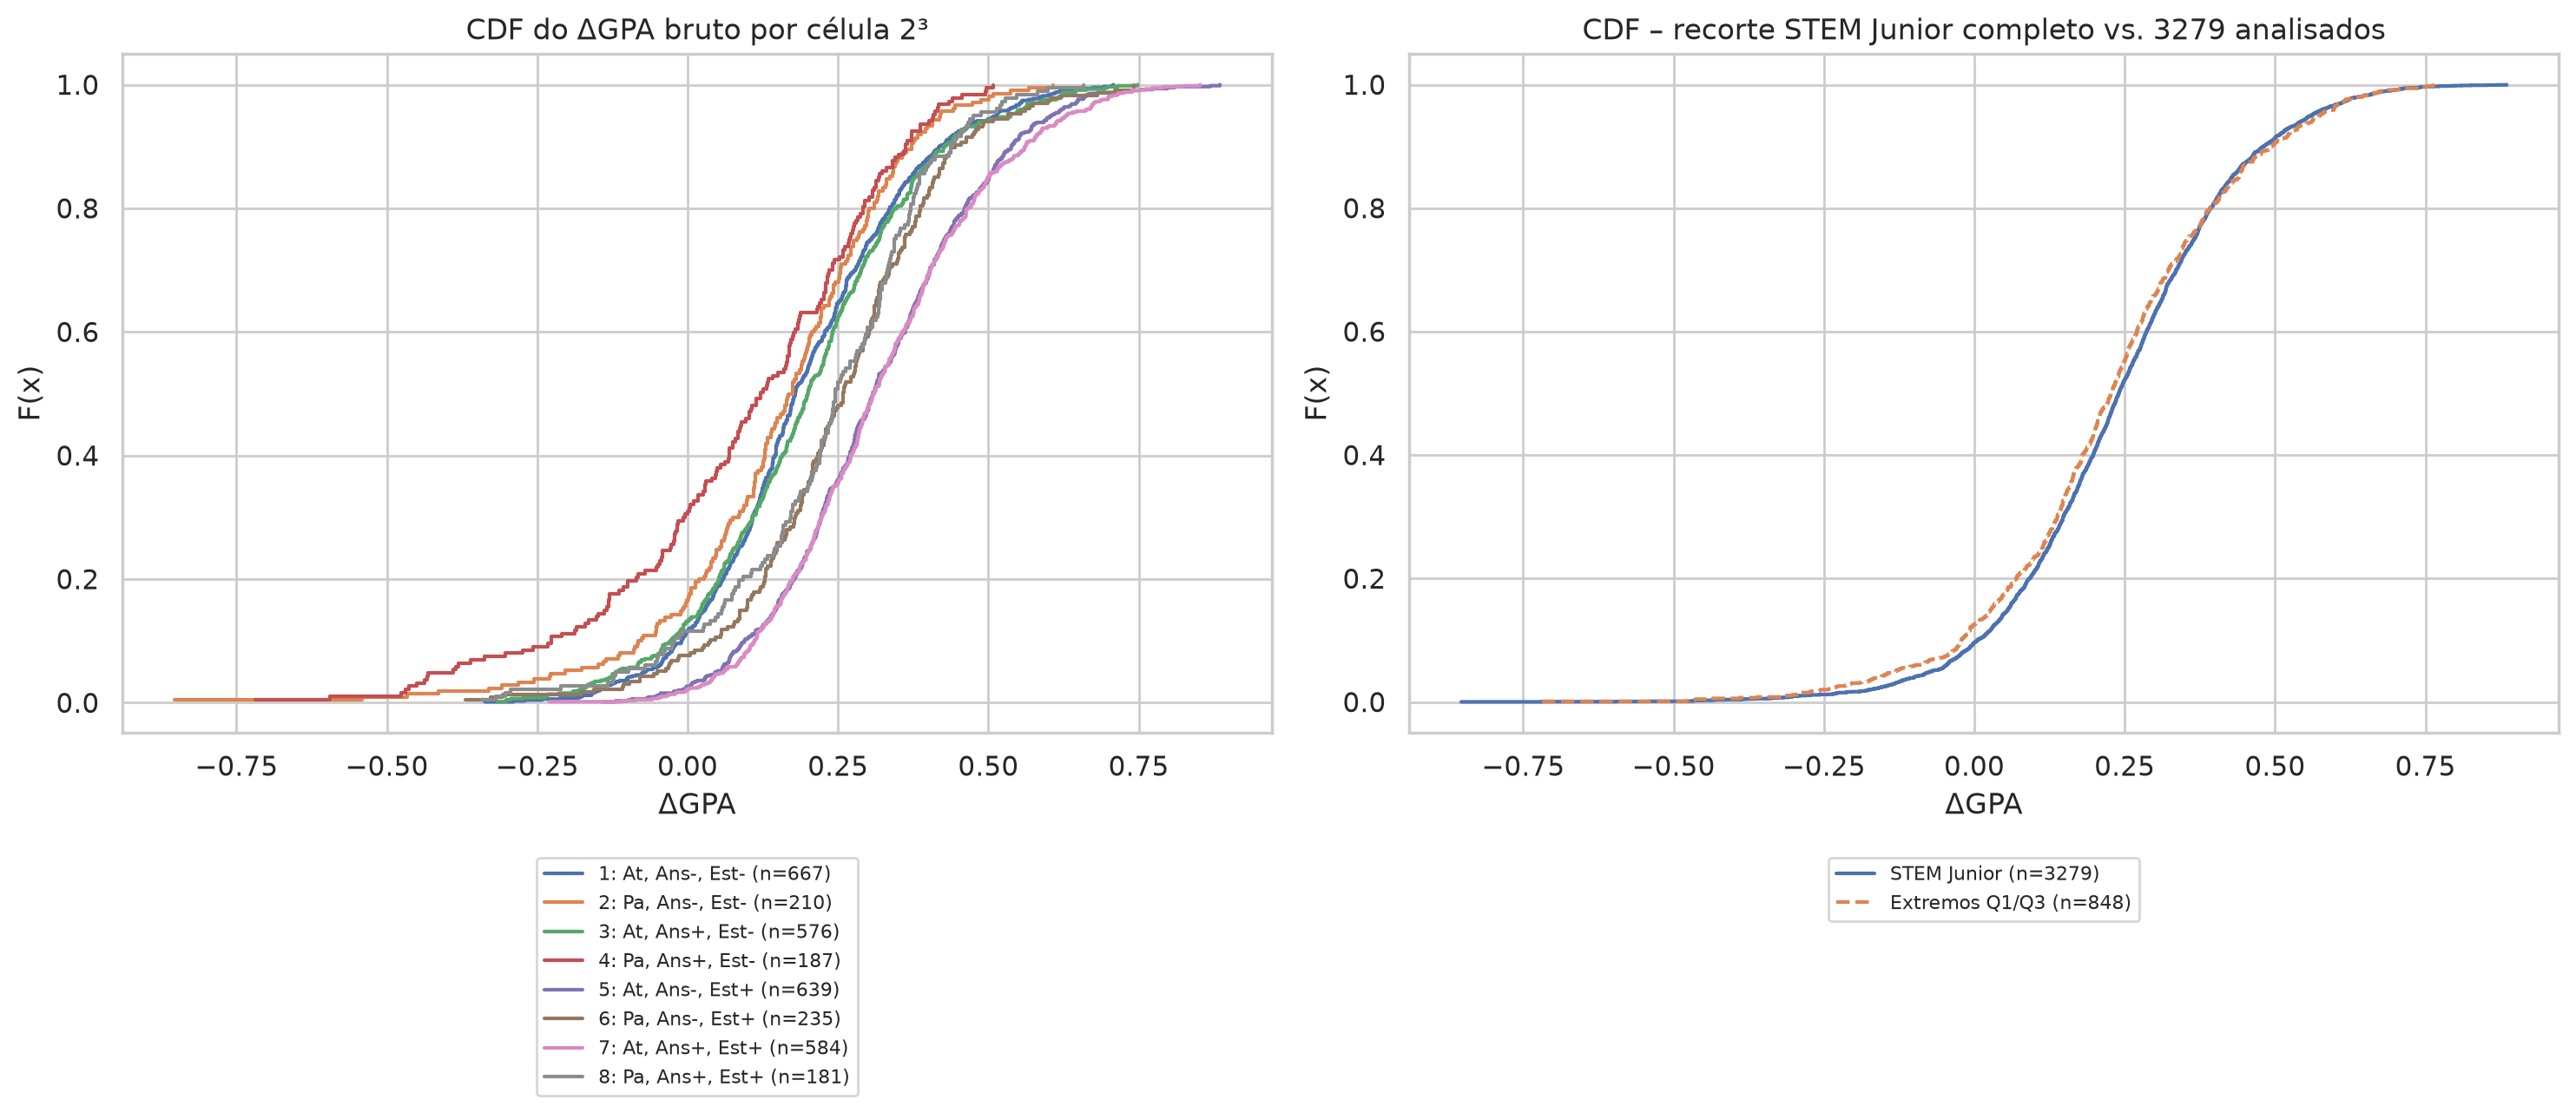
\includegraphics[width=\textwidth]{16_cdf_por_celula_e_recorte.png}
\caption{CDF do \dgpa{} por c\'elula e comparação do recorte analisado (n=3.279) com o subconjunto de extremos $Q_1/Q_3$.}\label{fig:cdf2}
\end{figure}

\begin{figure}[H]\centering
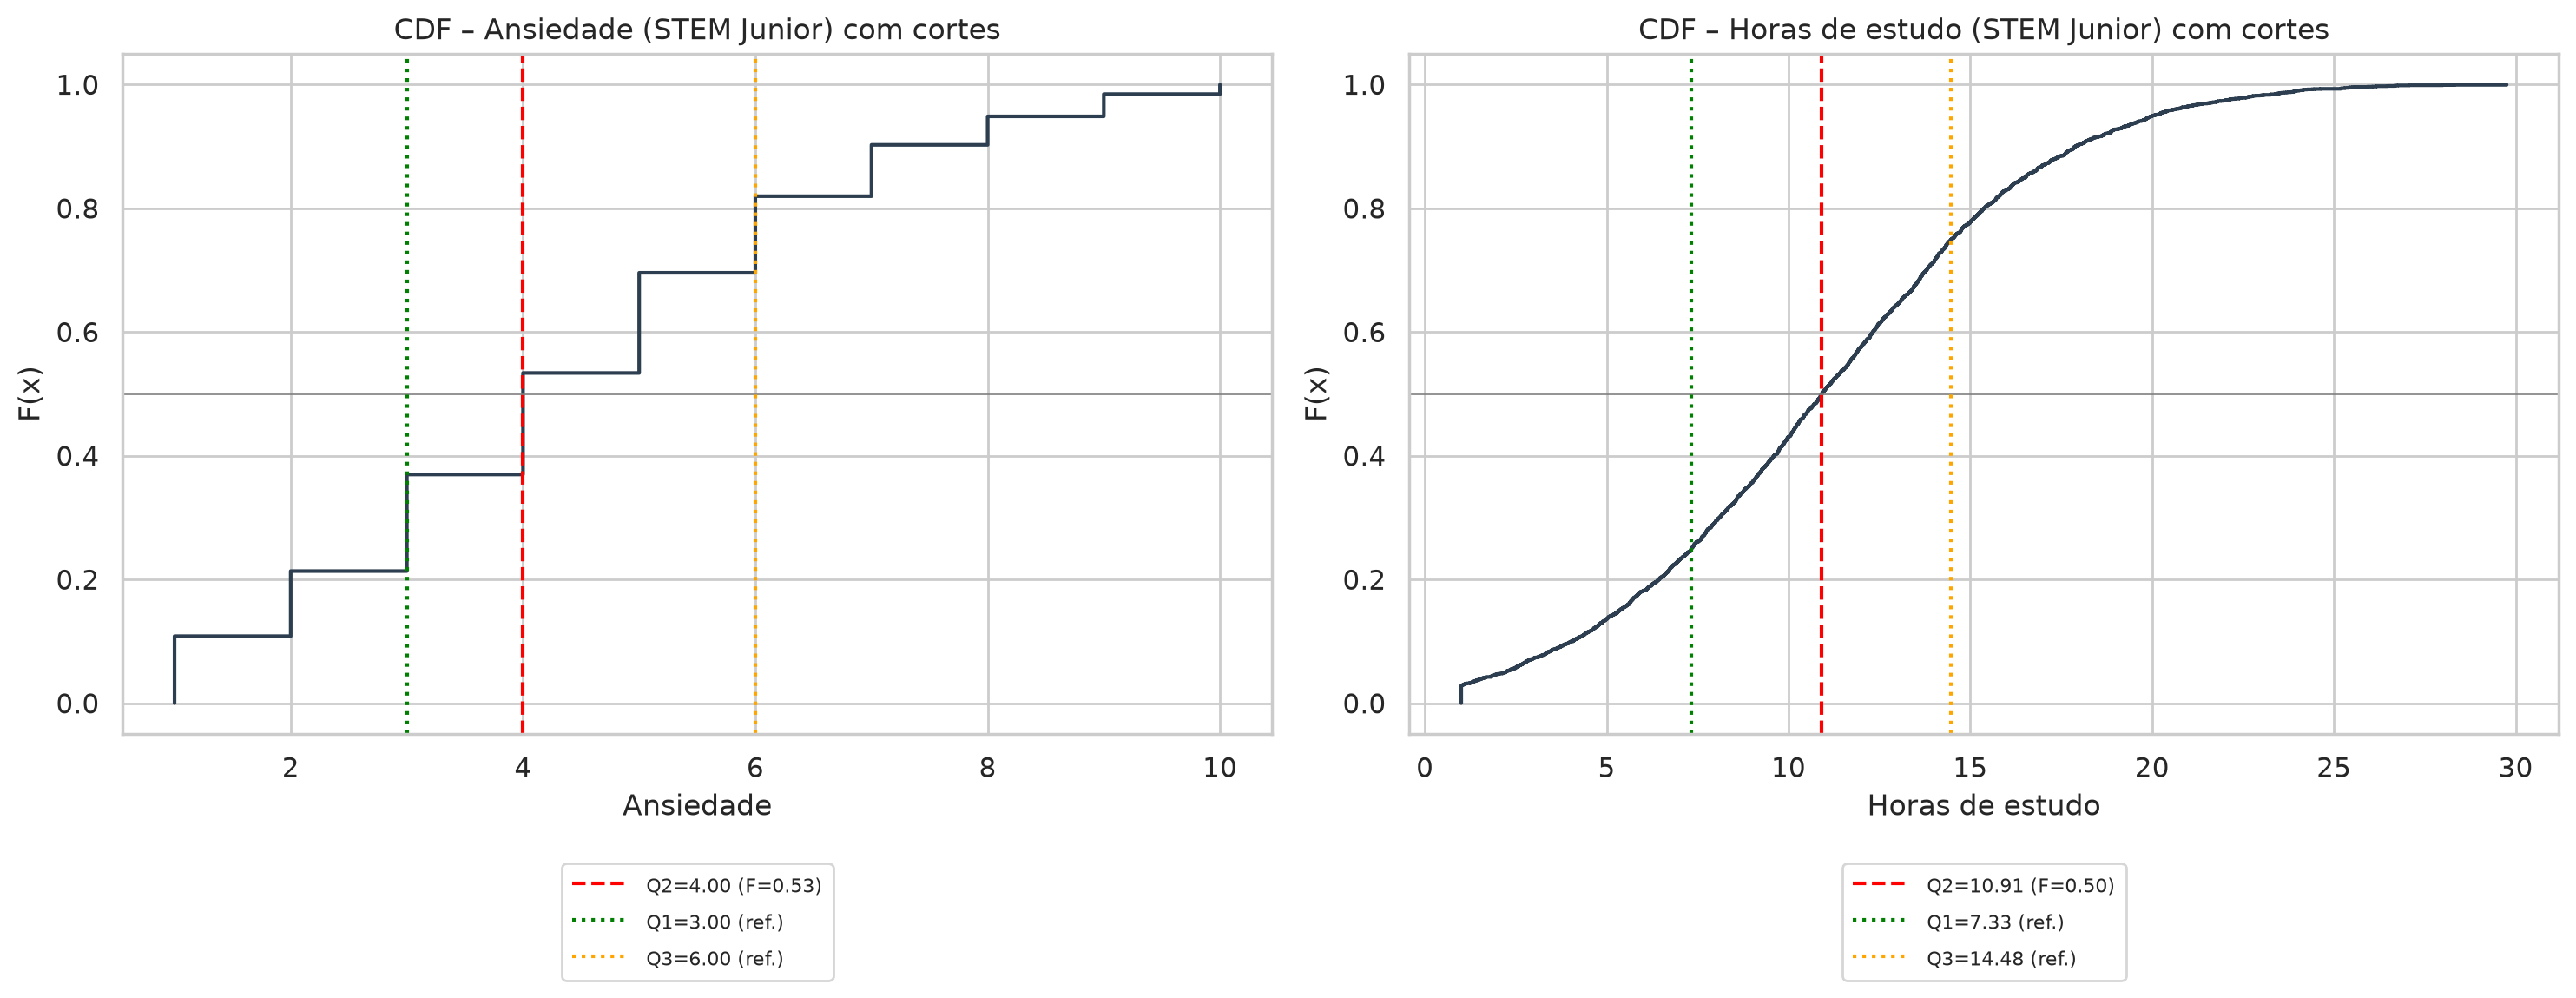
\includegraphics[width=\textwidth]{17_cdf_ansiedade_horas_quartis.png}
\caption{CDF de ansiedade e horas de estudo com marca\c{c}\~ao de $Q_2$ (corte) e de $Q_1$, $Q_3$ (refer\^encia).}\label{fig:cdf3}
\end{figure}

\subsection{Resposta bruta por c\'elula}
A Figura~\ref{fig:box} exibe o \dgpa{} bruto por c\'elula. As c\'elulas passivas t\^em assimetria negativa
(de $-0{,}72$ a $-1{,}13$; Shapiro--Wilk $p<0{,}001$ nas c\'elulas 2, 4 e 8), em parte pelo teto de GPA 4,0, o que motiva a normaliza\c{c}\~ao via bootstrap.
As c\'elulas passivas tamb\'em t\^em maior dispers\~ao (DP at\'e 0,236 contra cerca de 0,17).
O balanceamento da covari\'avel \texttt{Pre\_Semester\_GPA} entre as c\'elulas \'e adequado (ANOVA, $p=0{,}89$).

\begin{figure}[H]\centering
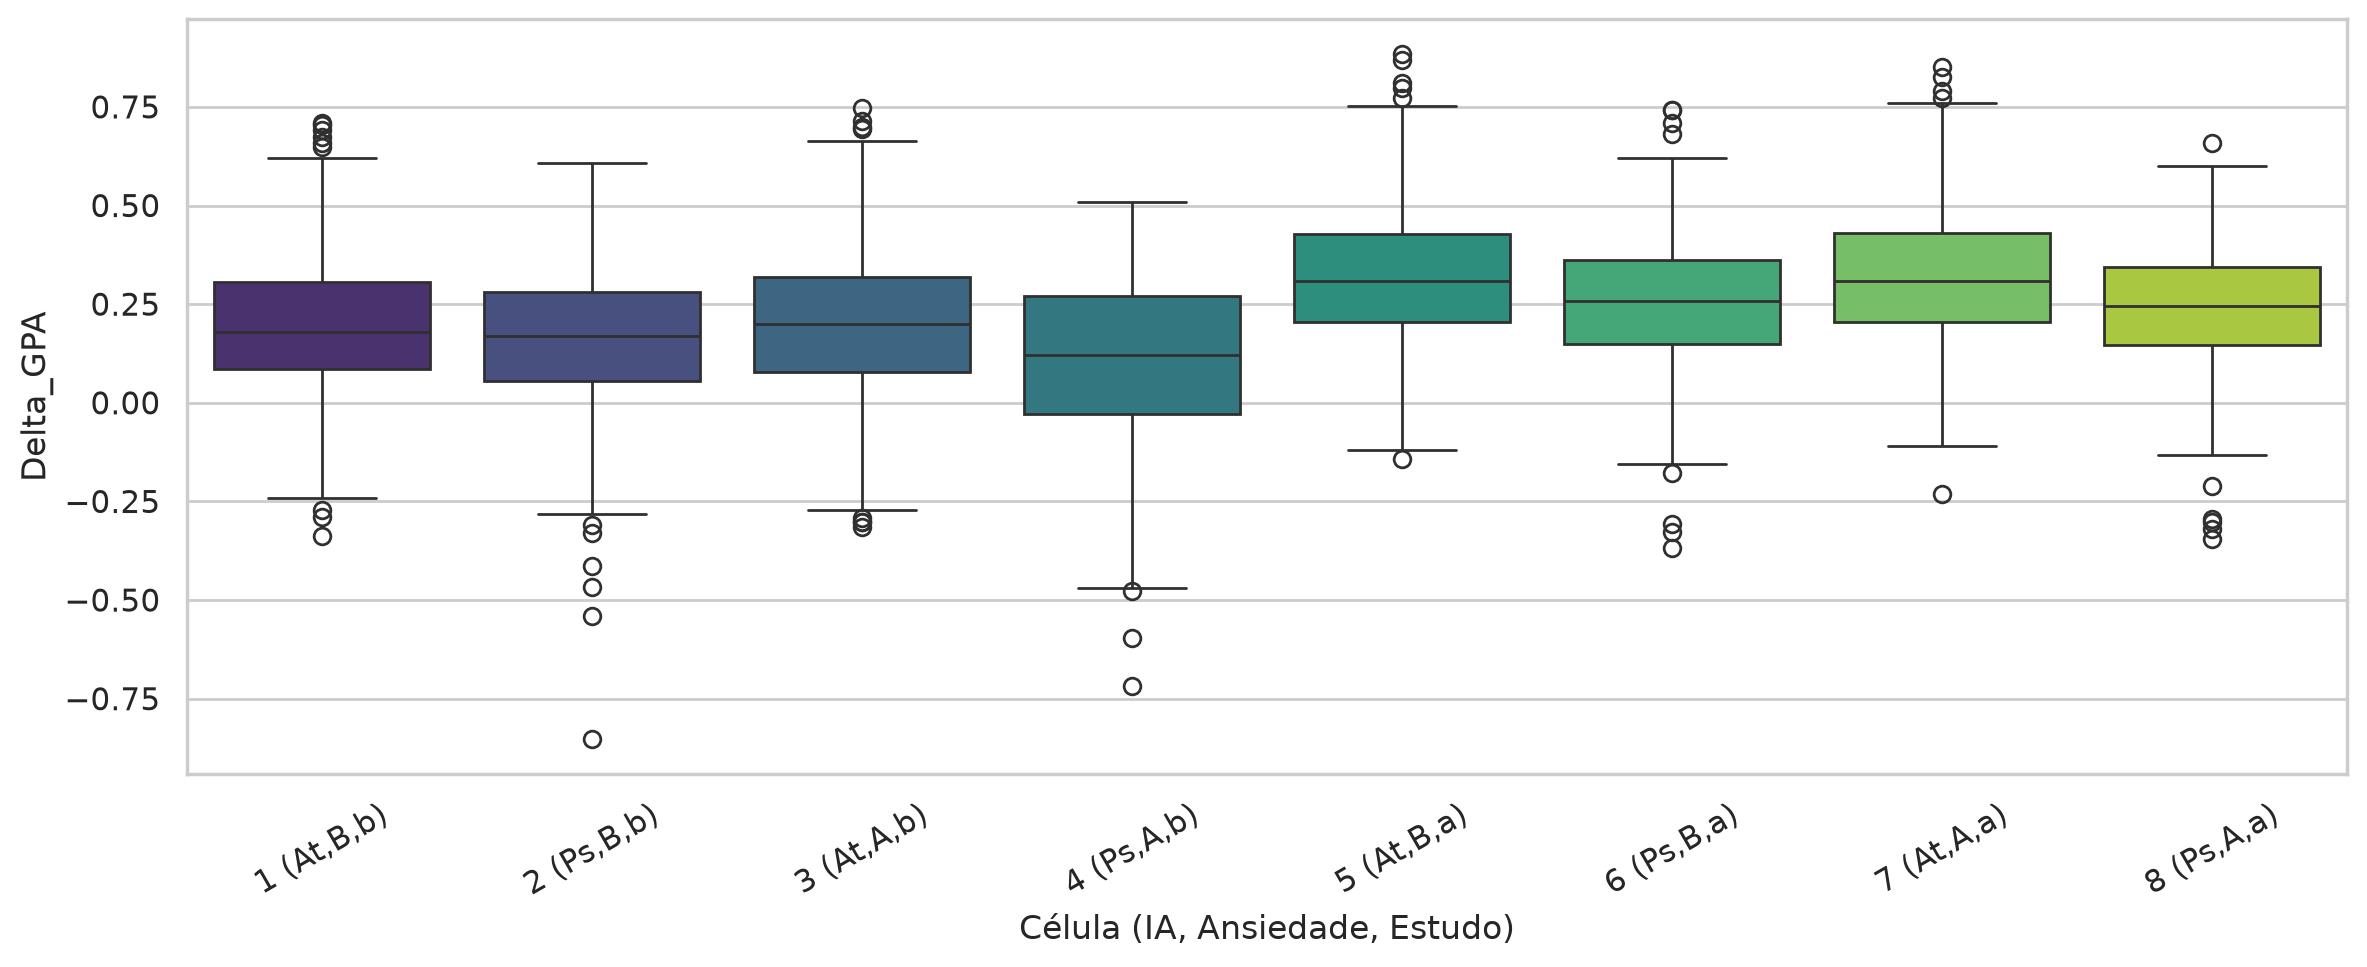
\includegraphics[width=\textwidth]{03_boxplot_bruto_por_celula.png}
\caption{\dgpa{} bruto por c\'elula experimental.}\label{fig:box}
\end{figure}

%=====================================================================
\section{Materiais e M\'etodos}
%=====================================================================
\subsection{Ambiente}
Python 3.12.3, NumPy 2.5.4, pandas 3.1.0, SciPy 1.18.1, statsmodels 1.18.1, Matplotlib 3.11.2 e seaborn 0.15.0.
O c\'odigo (\texttt{pcc170\_entrega02.py}) e o notebook executado (\texttt{.ipynb}) acompanham o relat\'orio.
Sementes: 42 (principal) e outras nove para checar estabilidade.

\subsection{Unidade experimental, fatores, n\'iveis e resposta}
\textbf{Unidade experimental:} aluno de STEM no 3.\textordmasculine{} ano (\emph{Junior}). \textbf{Resposta:} \dgpa{}.
\textbf{Condi\c{c}\~oes controladas:} \'area (STEM) e ano de estudo fixos; \texttt{Pre\_GPA} verificado como balanceado.
Os fatores B e C s\~ao dicotomizados pela mediana; essa escolha \'e comparada com a regra por quartis extremos e com um modelo cont\'inuo na an\'alise de sensibilidade.

\begin{table}[H]
\centering
\caption{Fatores e n\'iveis.}
\begin{tabular}{llp{5.2cm}p{4cm}}
\toprule
Fator & Nome & N\'ivel $-1$ & N\'ivel $+1$\\
\midrule
A & Modo de uso da IA & Ativo (Ideation, Summarizing, Debugging) & Passivo (Copywriting/Drafting, Direct Answer)\\
B & Ansiedade em exames & Baixa ($\le 4$) & Alta ($>4$)\\
C & Horas de estudo & Baixas ($\le 10{,}91$) & Altas ($>10{,}91$)\\
\bottomrule
\end{tabular}
\end{table}

\subsection{Quadro das combina\c{c}\~oes de teste}
Os 8 ensaios seguem a ordem de Yates (A varia mais r\'apido). A Tabela~\ref{tab:comb} apresenta as combina\c{c}\~oes,
os tamanhos de c\'elula e as estat\'isticas da resposta; a Tabela~\ref{tab:sinais} traz a matriz de sinais
com colunas A, B, C, AB, AC, BC e ABC (produto dos sinais), usada para calcular os efeitos.
A Figura~\ref{fig:quadros} reproduz ambos os quadros.

\begin{table}[H]
\centering
\caption{Combina\c{c}\~oes de teste (ordem de Yates).}\label{tab:comb}
\begin{tabular}{ccccrcc}
\toprule
Ensaio & A & B & C & $n$ & M\'edia \dgpa{} & DP\\
\midrule
(1) & $-$ & $-$ & $-$ & 667 & 0,196 & 0,172\\
a   & $+$ & $-$ & $-$ & 210 & 0,152 & 0,198\\
b   & $-$ & $+$ & $-$ & 576 & 0,201 & 0,184\\
ab  & $+$ & $+$ & $-$ & 187 & 0,091 & 0,236\\
c   & $-$ & $-$ & $+$ & 639 & 0,317 & 0,170\\
ac  & $+$ & $-$ & $+$ & 235 & 0,252 & 0,176\\
bc  & $-$ & $+$ & $+$ & 584 & 0,323 & 0,173\\
abc & $+$ & $+$ & $+$ & 181 & 0,233 & 0,179\\
\bottomrule
\end{tabular}
\end{table}

\begin{table}[H]
\centering
\caption{Matriz de sinais dos efeitos.}\label{tab:sinais}
\begin{tabular}{c|ccccccc}
\toprule
Ensaio & A & B & C & AB & AC & BC & ABC\\
\midrule
(1) & $-$ & $-$ & $-$ & $+$ & $+$ & $+$ & $-$\\
a   & $+$ & $-$ & $-$ & $-$ & $-$ & $+$ & $+$\\
b   & $-$ & $+$ & $-$ & $-$ & $+$ & $-$ & $+$\\
ab  & $+$ & $+$ & $-$ & $+$ & $-$ & $-$ & $-$\\
c   & $-$ & $-$ & $+$ & $+$ & $-$ & $-$ & $+$\\
ac  & $+$ & $-$ & $+$ & $-$ & $+$ & $-$ & $-$\\
bc  & $-$ & $+$ & $+$ & $-$ & $-$ & $+$ & $-$\\
abc & $+$ & $+$ & $+$ & $+$ & $+$ & $+$ & $+$\\
\bottomrule
\end{tabular}
\end{table}

\begin{figure}[H]\centering
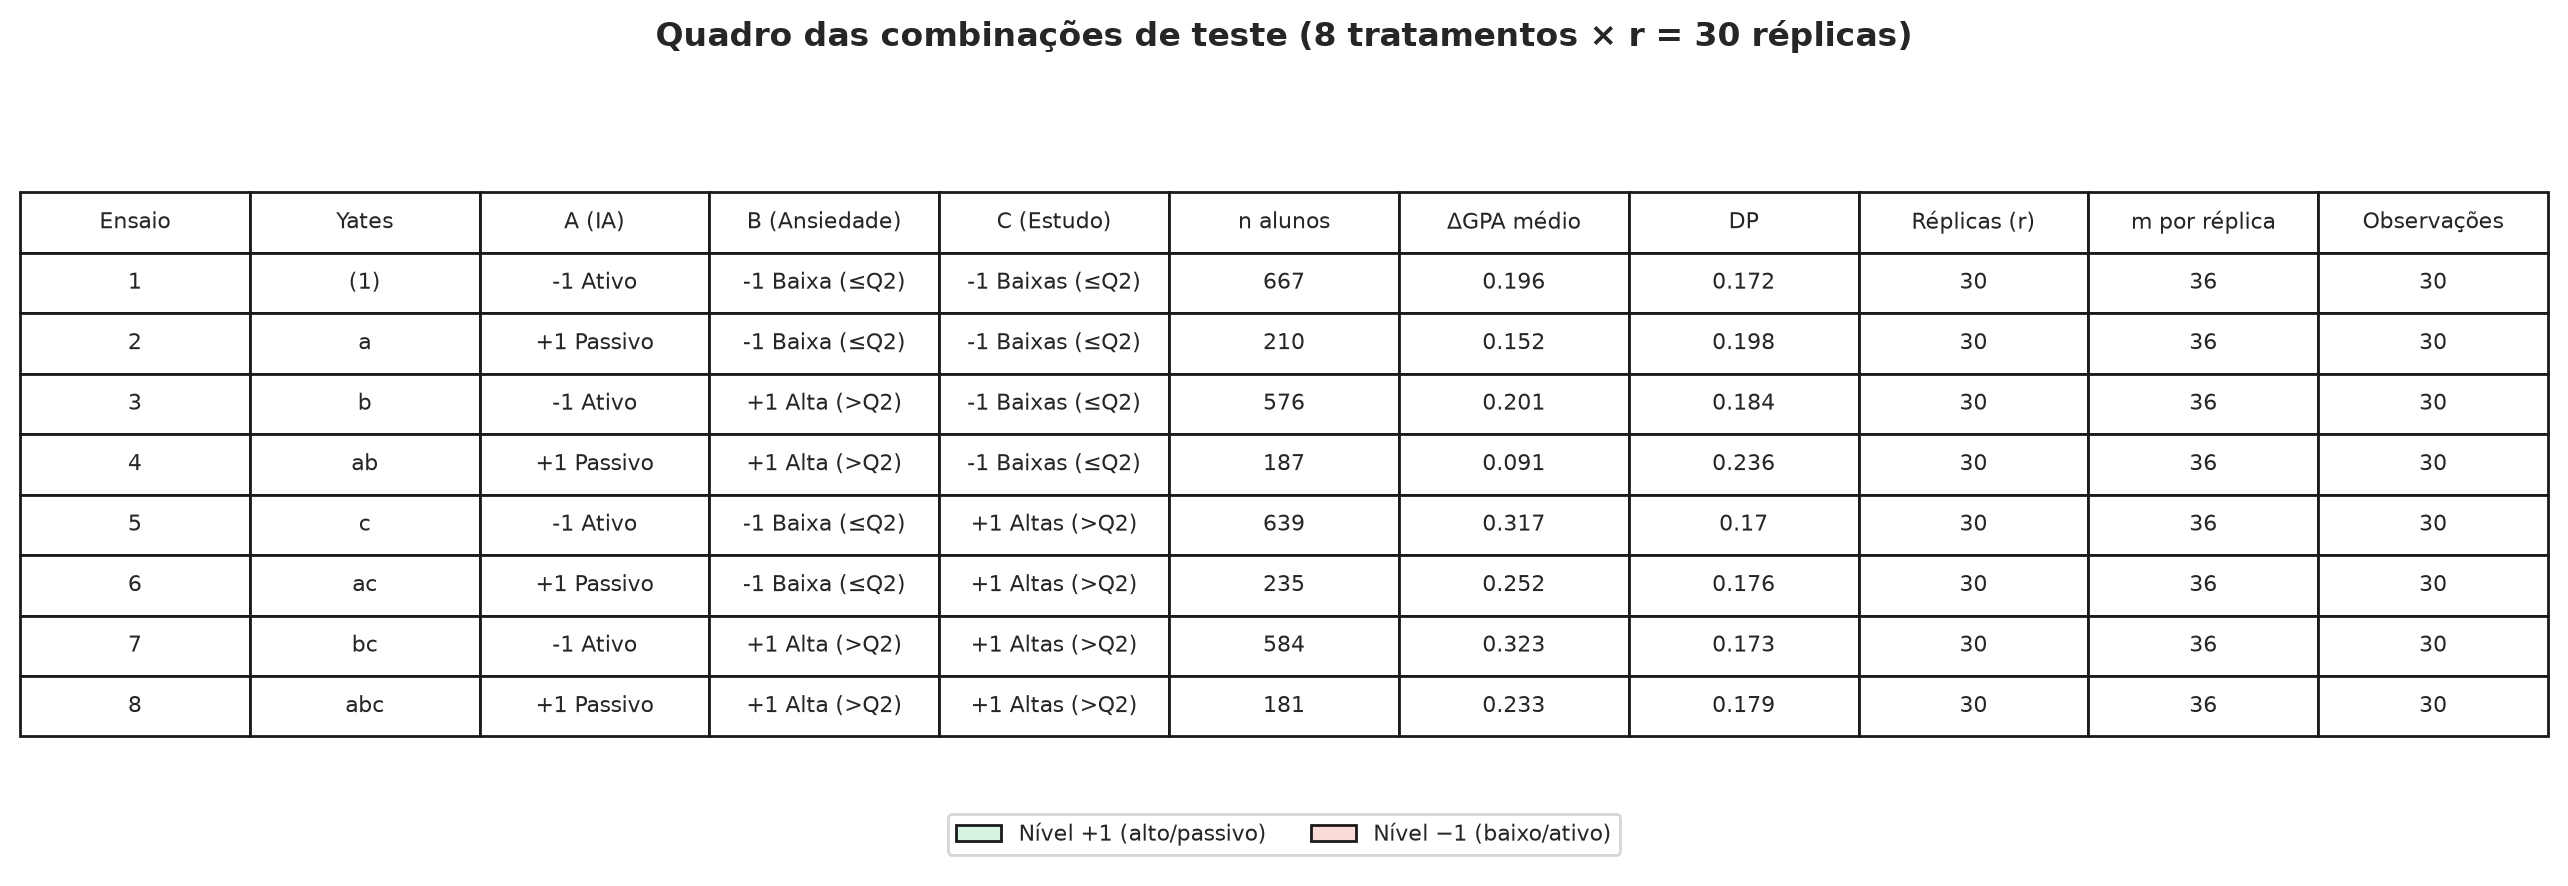
\includegraphics[width=\textwidth]{19a_quadro_combinacoes_teste.png}
\caption{Quadro das combina\c{c}\~oes de teste.}\label{fig:quadros}
\end{figure}
\begin{figure}[H]\centering
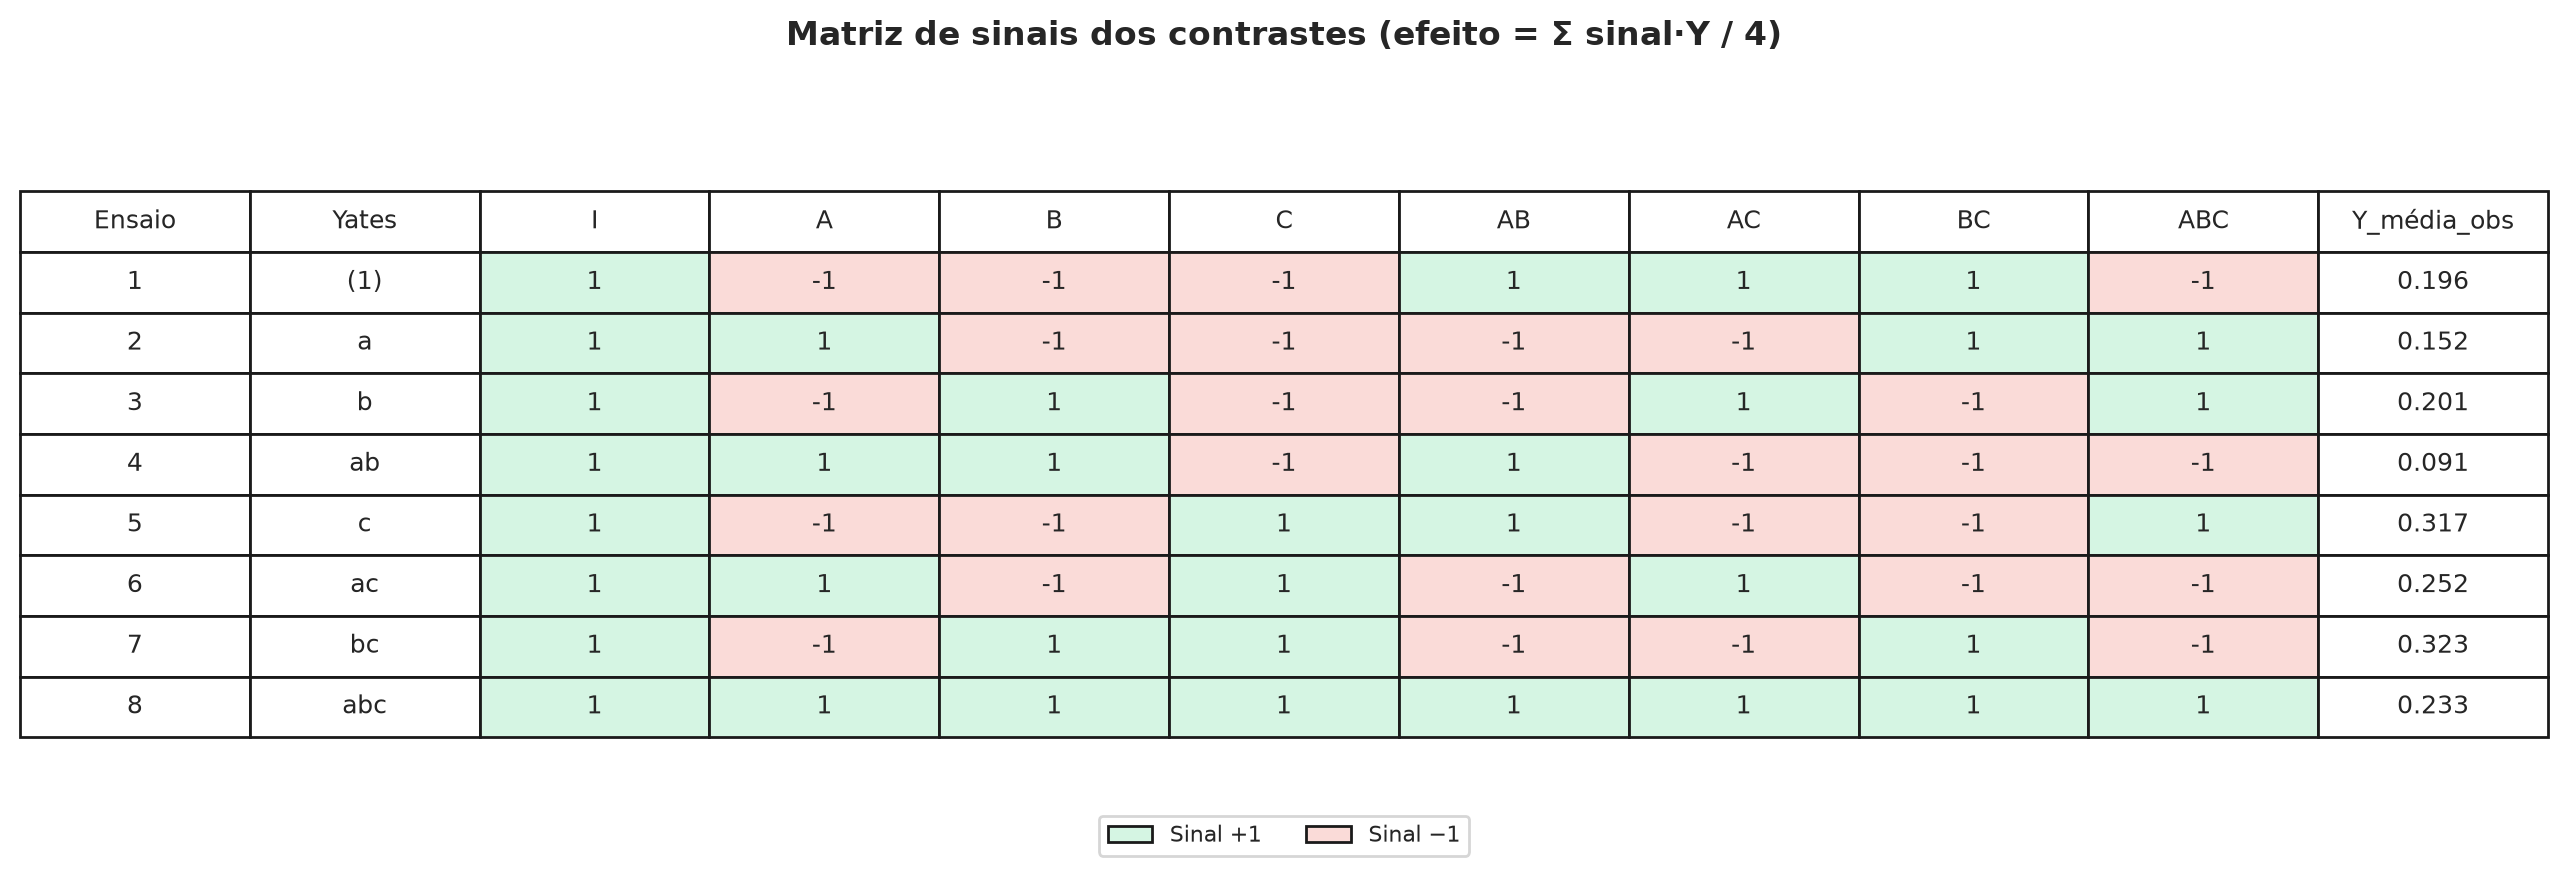
\includegraphics[width=\textwidth]{19b_matriz_sinais_contrastes.png}
\caption{Matriz de sinais dos contrastes.}\label{fig:sinais}
\end{figure}

\subsection{Modelo principal: ANOVA $2^3$ sobre os dados brutos}
Os alunos s\~ao as unidades experimentais e as $n=3.279$ observa\c{c}\~oes brutas s\~ao o ``experimento'' (fatorial $2^3$ observacional e n\~ao balanceado,
com $n_c=181$--$667$ por c\'elula). Ajusta-se \texttt{$\Delta$GPA $\sim$ A*B*C} com codifica\c{c}\~ao $\pm1$, SQ tipo III (testa exatamente o contraste de efeito, mesmo com $n$ desigual)
e erros-padr\~ao robustos \`a heterocedasticidade (HC3). Essa \'e a \'unica fonte de $p$-valores da decis\~ao.

\subsection{Efeitos e intervalos de confian\c{c}a (bootstrap estratificado)}
O efeito de cada termo \'e
\[
\text{efeito}=\frac{1}{4}\sum_{c=1}^{8} s_c\,\overline{Y}_c ,
\]
onde $s_c$ \'e o sinal da coluna correspondente (Tabela~\ref{tab:sinais}) e $\overline{Y}_c$ a m\'edia bruta da c\'elula; equivale ao dobro do coeficiente
da regress\~ao com vari\'aveis codificadas em $\pm1$. O bootstrap \'e usado \emph{exclusivamente} para os ICs: 5.000 reamostras estratificadas (tamanho $n_c$ completo
de cada c\'elula), recalculando os sete efeitos e obtendo ICs de 95\% pelo m\'etodo percentil, que n\~ao assumem vari\^ancias iguais.

\subsection{R\'eplicas bootstrap: papel apenas ilustrativo}
Sortear $m=36$ alunos \emph{com reposi\c{c}\~ao} de cada c\'elula $r=30$ vezes (240 m\'edias) ilustra o balanceamento e a normaliza\c{c}\~ao das m\'edias pelo Teorema Central do Limite,
mas \textbf{n\~ao constitui replica\c{c}\~ao experimental}: as r\'eplicas reamostram os mesmos alunos (pseudo-replica\c{c}\~ao) e medem a variabilidade do estimador, n\~ao o erro experimental.
Por isso a ANOVA sobre essas m\'edias tem $p$-valores otimistas e n\~ao \'e usada para decidir (Ap\^endice~A).

\subsection{Crit\'erios de valida\c{c}\~ao e decis\~ao}
\begin{itemize}
\item Diagn\'ostico dos res\'iduos do modelo bruto: Shapiro--Wilk, Levene e gr\'afico res\'iduos $\times$ ajustados. Em caso de heterocedasticidade, o modelo adota HC3 e confere-se o IC bootstrap.
\item Estabilidade: desvio-padr\~ao do efeito entre 10 sementes $<0{,}01$ (Ap\^endice~A).
\item Balanceamento de \texttt{Pre\_GPA} (ANOVA, $p>0{,}05$).
\item Decis\~ao: efeito \emph{significativo} se o IC95\% bootstrap exclui 0 \textbf{e} o $p$ (HC3) do modelo bruto $<0{,}05$;
\emph{fraco} se apenas um dos crit\'erios \'e atendido; \emph{n\~ao significativo} caso contr\'ario.
\end{itemize}

%=====================================================================
\section{Resultados Experimentais}
%=====================================================================
\subsection{Vis\~ao geral das respostas (cubo)}
A Figura~\ref{fig:cubo} apresenta o \dgpa{} m\'edio nos oito v\'ertices. O pior v\'ertice \'e
\emph{passivo + ansiedade alta + pouco estudo} ($0{,}091$); o melhor, \emph{ativo + ansiedade alta + muito estudo} ($0{,}323$),
praticamente empatado com \emph{ativo + ansiedade baixa + muito estudo} ($0{,}317$).

\begin{figure}[H]\centering
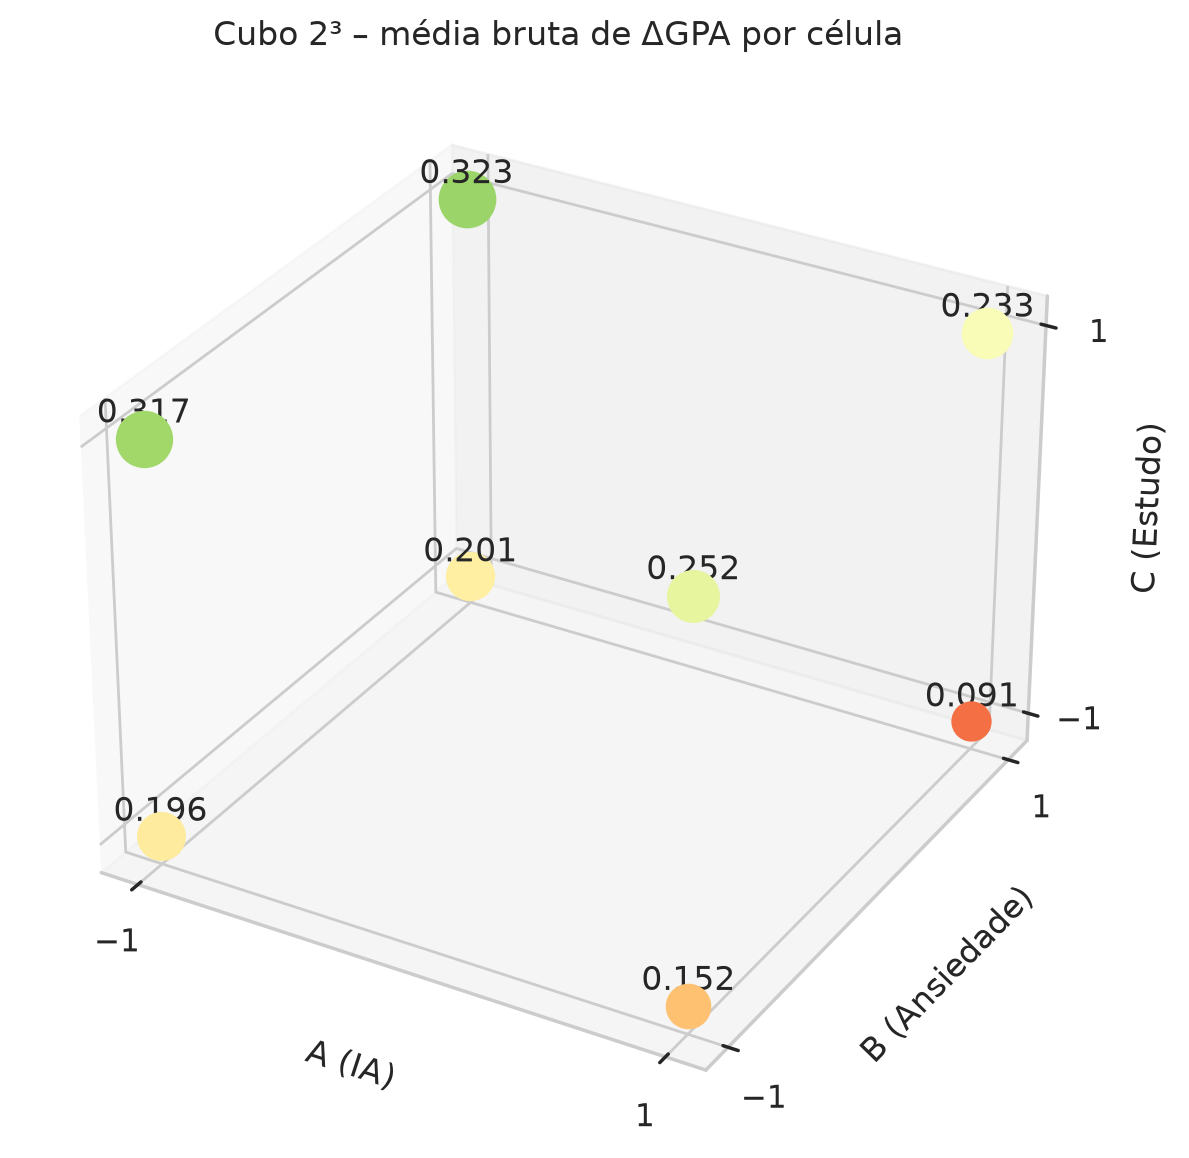
\includegraphics[width=0.8\textwidth]{07_cubo_2x3.png}
\caption{\dgpa{} m\'edio por v\'ertice do cubo $2^3$.}\label{fig:cubo}
\end{figure}

\subsection{ANOVA do fatorial $2^3$ sobre os dados brutos (HC3)}
\begin{table}[H]
\centering
\caption{ANOVA $2^3$ n\~ao balanceada ($n=3.279$; SQ tipo III; $p$ cl\'assico e com erros-padr\~ao HC3). Res\'iduo: 89,0\% da SQ total ($R^2=0{,}129$).}
\begin{tabular}{lrrrrr}
\toprule
Fonte & SQ & $F$ (cl\'assico) & $p$ cl\'assico & $p$ (HC3) & \% da SQ total\\
\midrule
A & 3,608 & 110,7 & $<0{,}001$ & $<0{,}001$ & 3,01\\
B & 0,185 & 5,69 & 0,017 & 0,027 & 0,15\\
C & 8,894 & 272,9 & $<0{,}001$ & $<0{,}001$ & 7,43\\
AB & 0,311 & 9,54 & 0,002 & 0,004 & 0,26\\
AC & 0,0001 & 0,004 & 0,947 & 0,951 & $<0{,}01$\\
BC & 0,069 & 2,12 & 0,146 & 0,177 & 0,06\\
ABC & 0,057 & 1,76 & 0,185 & 0,218 & 0,05\\
Res\'iduo & 106,589 & -- & -- & -- & 89,0\\
\bottomrule
\end{tabular}
\end{table}

Os fatores explicam 11\% da variabilidade individual do \dgpa{}, quase toda devida a C (7,4\%) e A (3,0\%); o restante \'e variabilidade entre alunos n\~ao explicada pelos tr\^es fatores (Figura~\ref{fig:pct}).

\begin{figure}[H]\centering
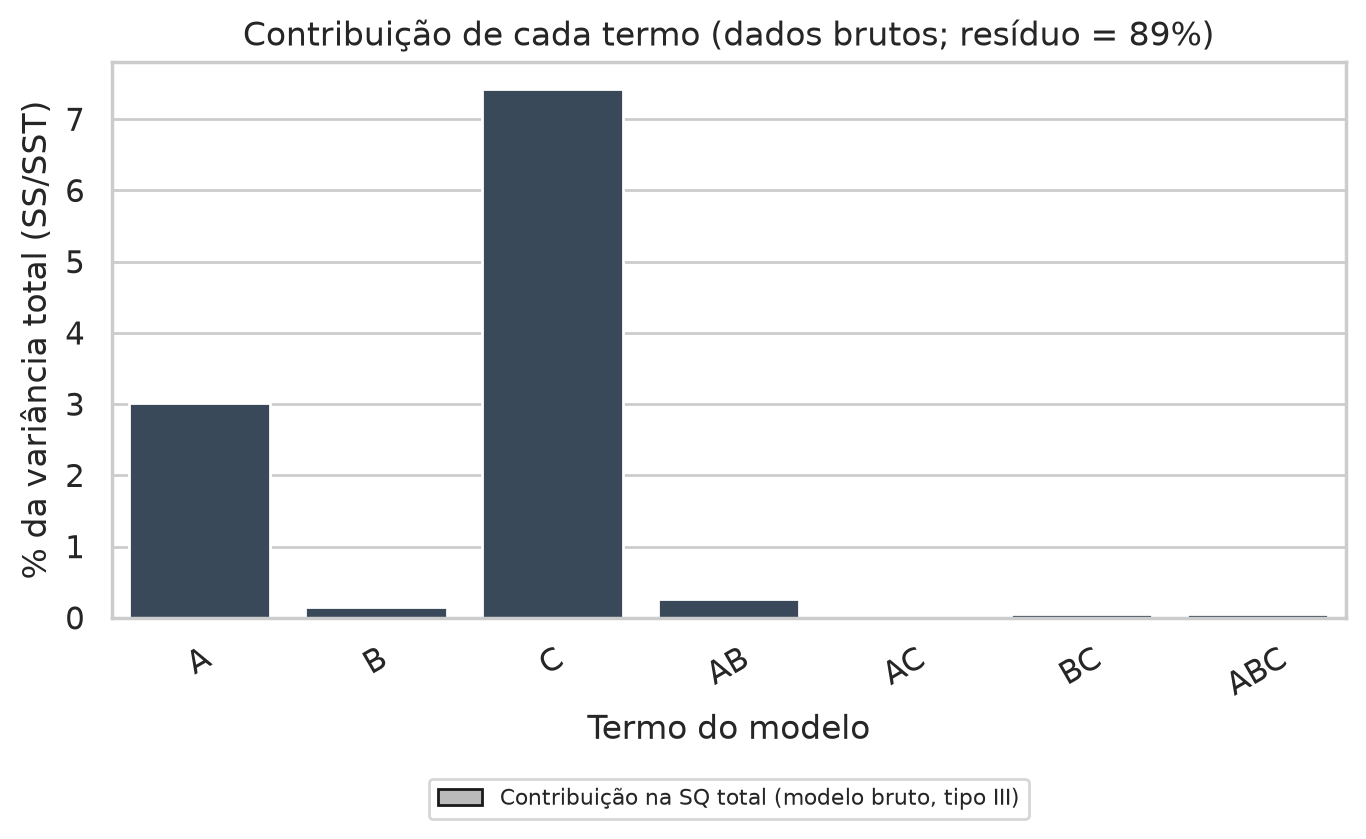
\includegraphics[width=0.85\textwidth]{13_pct_variancia.png}
\caption{Percentual da soma de quadrados total por termo (dados brutos).}\label{fig:pct}
\end{figure}

\subsection{Efeitos e intervalos de confian\c{c}a}
\begin{table}[H]
\centering
\caption{Efeitos estimados (m\'edias brutas), IC95\% bootstrap, $p$ (HC3) e veredito.}\label{tab:efeitos}
\begin{tabular}{lrcrl}
\toprule
Efeito & Valor & IC95\% & $p$ (HC3) & Veredito\\
\midrule
A (modo de uso) & $-0{,}0772$ & $[-0{,}0920;\,-0{,}0621]$ & $<0{,}001$ & significativo\\
B (ansiedade) & $-0{,}0175$ & $[-0{,}0329;\,-0{,}0019]$ & 0,027 & signif.\ (marginal)\\
C (horas) & $+0{,}1211$ & $[+0{,}1058;\,+0{,}1364]$ & $<0{,}001$ & significativo\\
AB & $-0{,}0226$ & $[-0{,}0384;\,-0{,}0074]$ & 0,004 & significativo\\
AC & $-0{,}0005$ & $[-0{,}0156;\,+0{,}0148]$ & 0,951 & n\~ao signif.\\
BC & $+0{,}0107$ & $[-0{,}0051;\,+0{,}0263]$ & 0,177 & n\~ao signif.\\
ABC & $+0{,}0097$ & $[-0{,}0063;\,+0{,}0253]$ & 0,218 & n\~ao signif.\\
\bottomrule
\end{tabular}
\end{table}

\begin{figure}[H]\centering
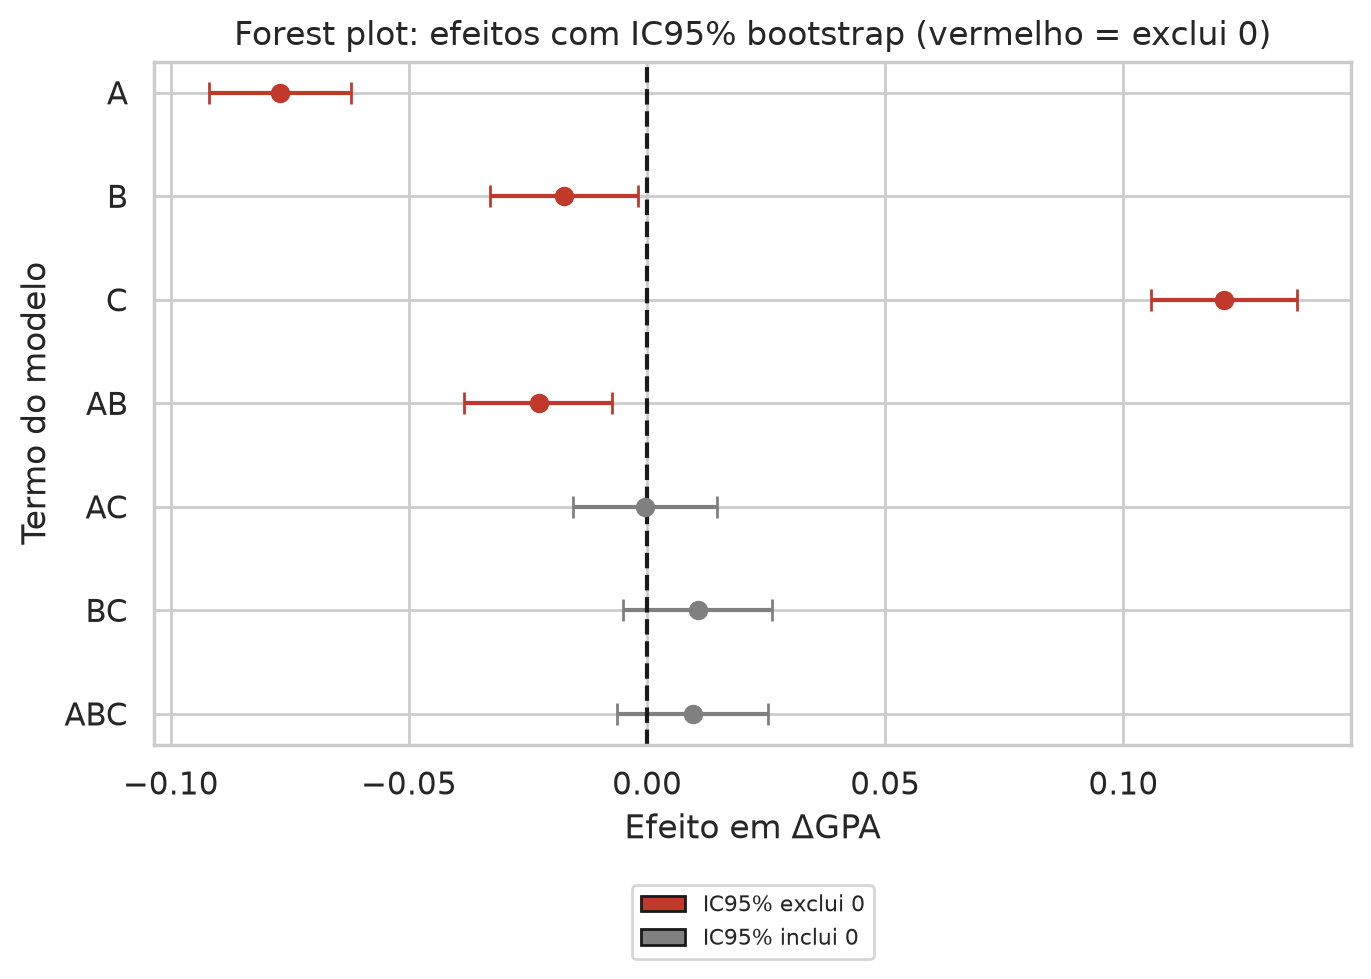
\includegraphics[width=0.9\textwidth]{12_forest_plot_efeitos.png}
\caption{\emph{Forest plot} dos efeitos com IC95\% bootstrap.}\label{fig:forest}
\end{figure}

\begin{figure}[H]\centering
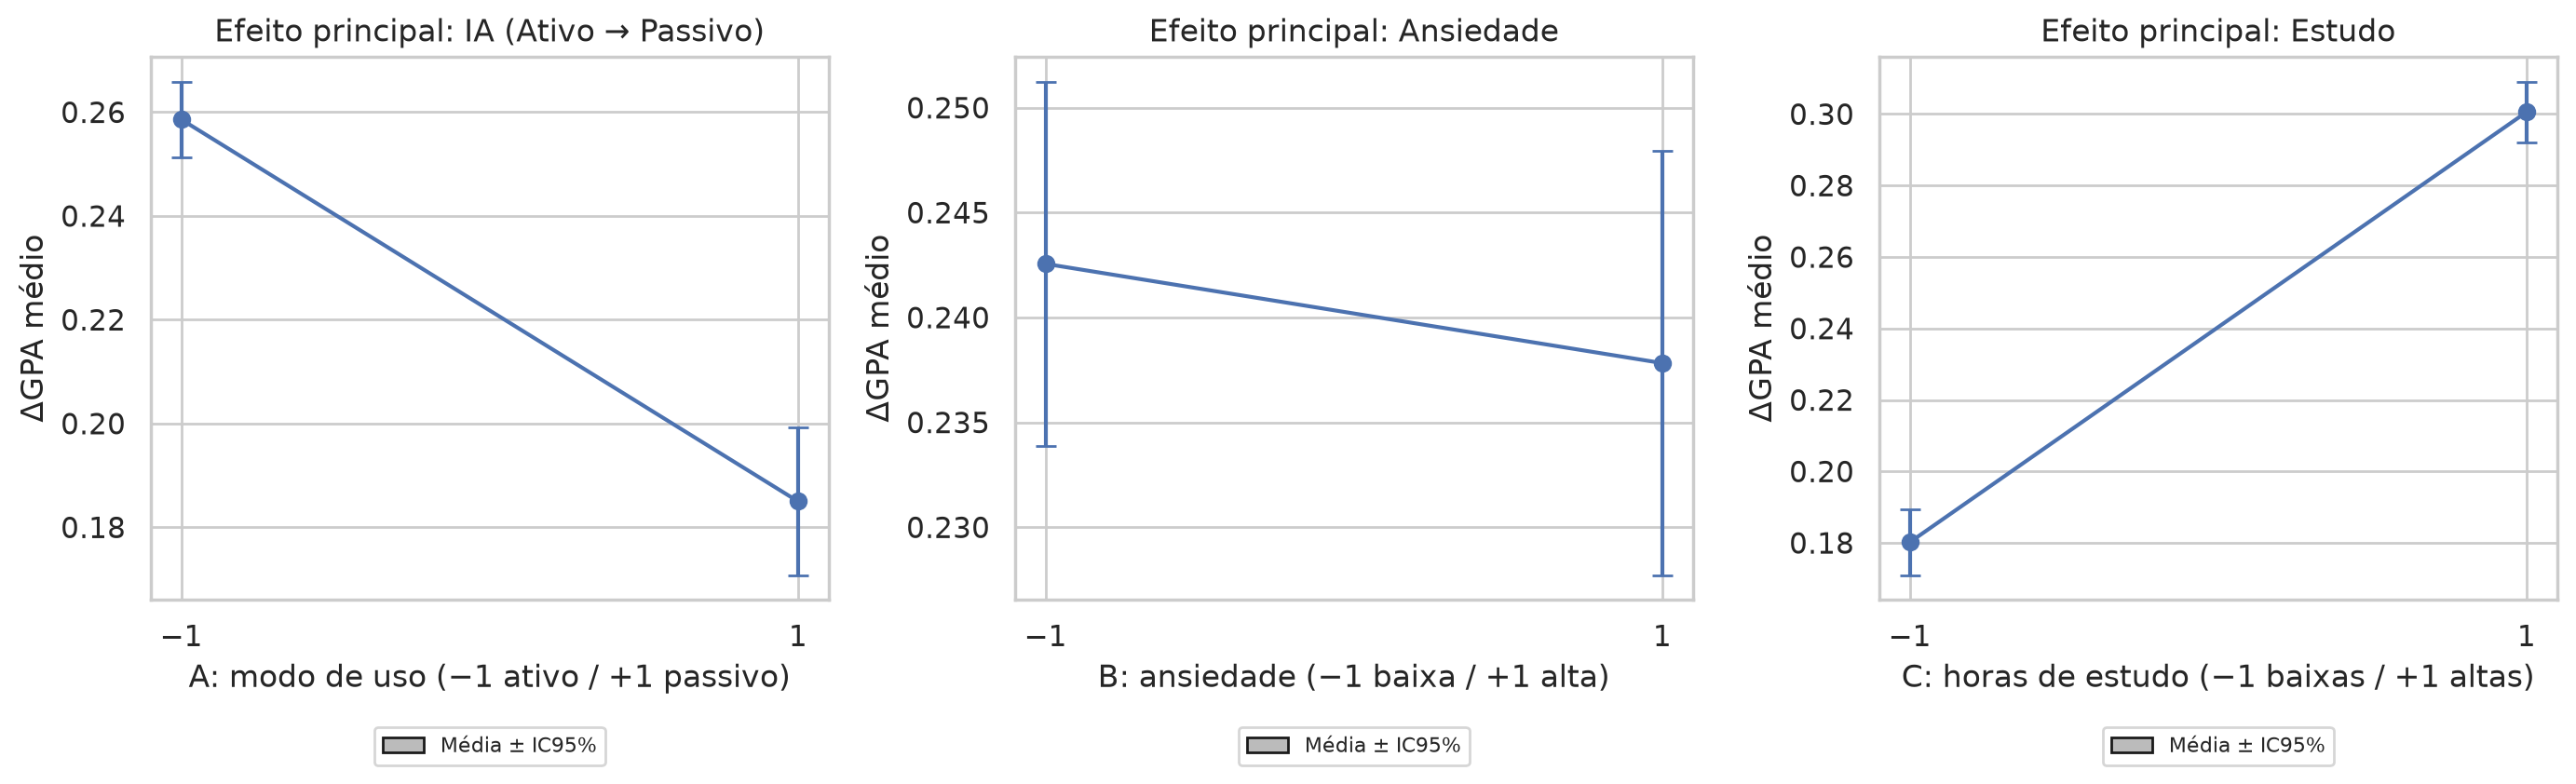
\includegraphics[width=0.9\textwidth]{08_efeitos_principais.png}
\caption{Efeitos principais sobre o \dgpa{}.}\label{fig:main}
\end{figure}

\begin{figure}[H]\centering
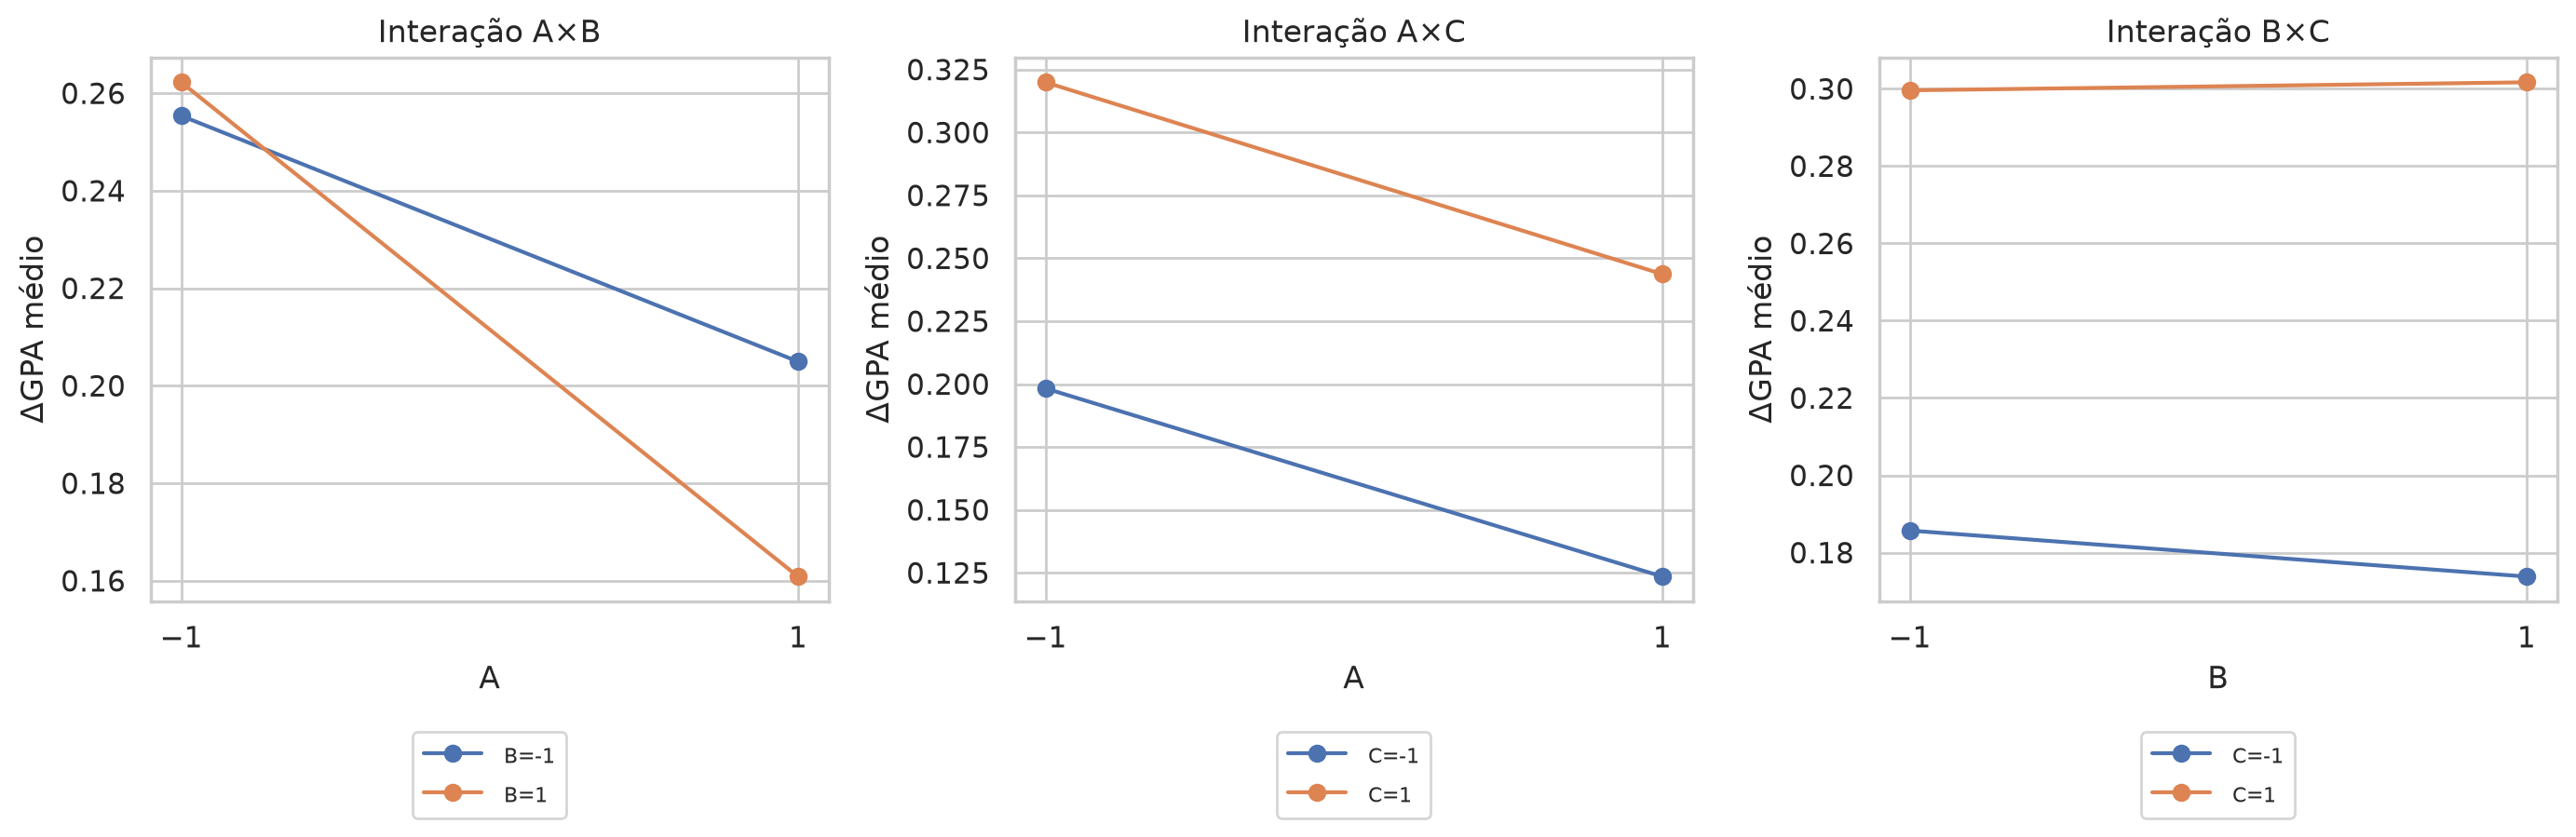
\includegraphics[width=\textwidth]{09_interacoes.png}
\caption{Gr\'aficos de intera\c{c}\~ao entre os fatores.}\label{fig:inter}
\end{figure}

\begin{figure}[H]\centering
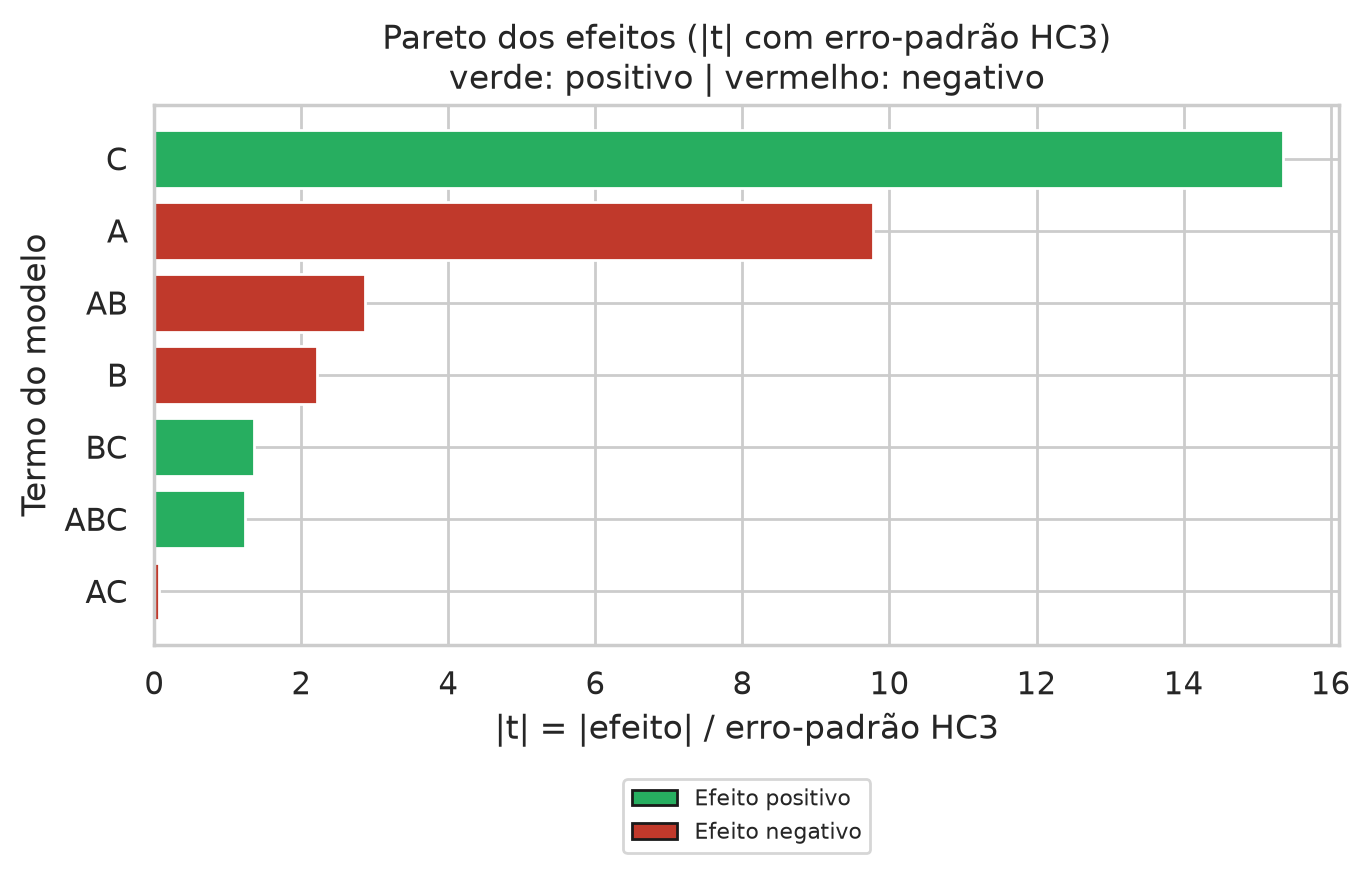
\includegraphics[width=0.9\textwidth]{10_pareto_efeitos.png}
\caption{Diagrama de Pareto dos efeitos ($|t|$ com erro-padr\~ao HC3).}\label{fig:pareto}
\end{figure}

\begin{figure}[H]\centering
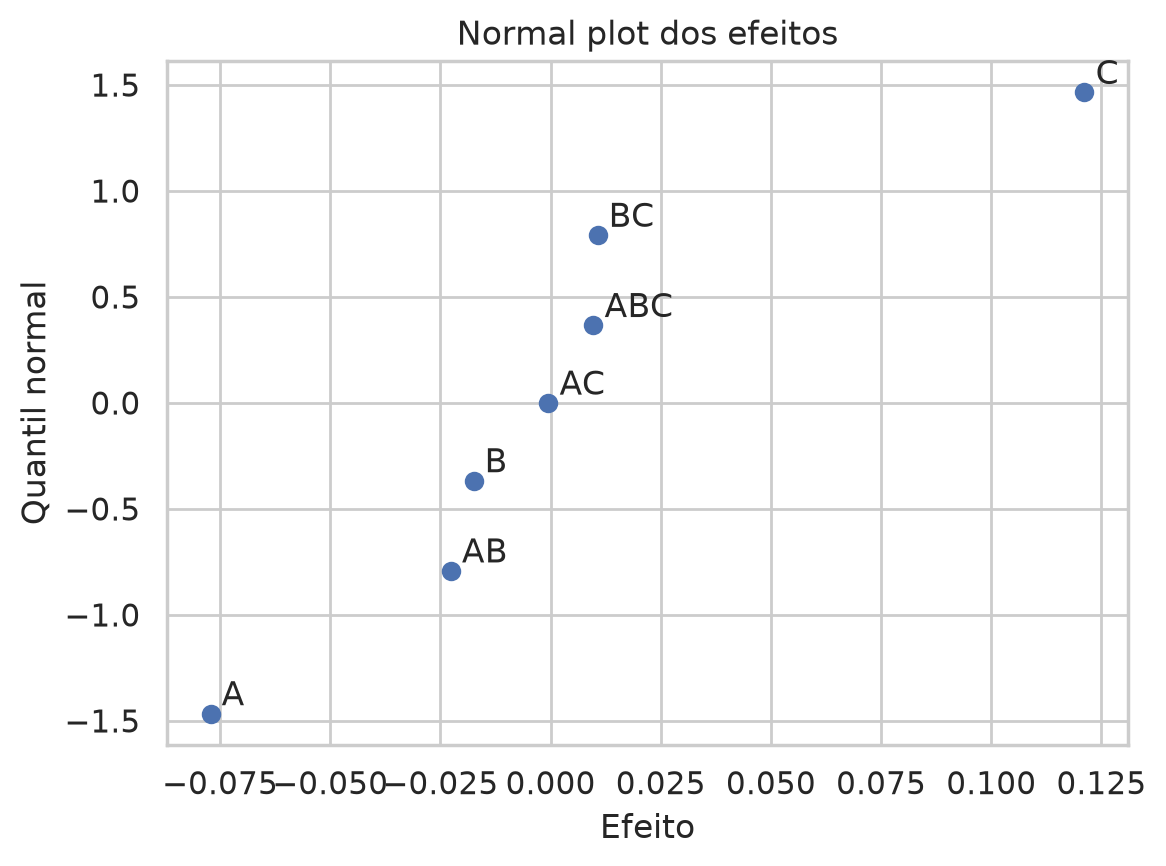
\includegraphics[width=0.8\textwidth]{11_normal_plot_efeitos.png}
\caption{Gr\'afico normal dos efeitos: pontos afastados da reta s\~ao efeitos ativos (C, A, AB e B).}\label{fig:normplot}
\end{figure}

\subsection{Diagn\'ostico dos res\'iduos e heterocedasticidade}
\begin{table}[H]
\centering
\caption{Checagens de valida\c{c}\~ao do modelo principal.}
\begin{tabular}{lcl}
\toprule
Checagem & Atendida & Detalhe\\
\midrule
Levene entre c\'elulas, dados brutos ($p>0{,}05$) & \textbf{N\~ao} & $p=2{,}6\times10^{-5}$ $\rightarrow$ HC3 + IC bootstrap\\
Concord\^ancia IC bootstrap $\times$ HC3 & Sim & os sete termos coincidem\\
Estabilidade entre sementes (DP $<0{,}01$) & Sim & DP m\'ax.\ $=0{,}0056$\\
Balanceamento de Pre\_GPA ($p>0{,}05$) & Sim & $p=0{,}89$\\
\bottomrule
\end{tabular}
\end{table}

\textbf{Heterocedasticidade.} O teste de Levene rejeita a homocedasticidade nos dados brutos ($p<0{,}001$): o DP por c\'elula varia de $0{,}170$ a $0{,}236$ e as c\'elulas passivas t\^em DP m\'edio maior ($0{,}197$) que as ativas ($0{,}175$), com o m\'aximo na c\'elula 4 (passivo, ansiedade alta, pouco estudo). Os res\'iduos s\~ao aproximadamente sim\'etricos, com cauda inferior (teto de GPA), e o gr\'afico res\'iduos $\times$ ajustados (Figura~\ref{fig:resid}) mostra dispers\~ao parecida entre c\'elulas, com pequenas diferen\c{c}as.
Em vez de transformar a resposta (a transforma\c{c}\~ao $\log Y$ da Aula~7 n\~ao se aplica, pois o \dgpa{} assume valores $\le0$), adotam-se estimadores robustos: ANOVA com matriz de covari\^ancia HC3 e ICs bootstrap, que n\~ao assumem vari\^ancias iguais. As duas abordagens concordam em todos os efeitos.

\begin{figure}[H]\centering
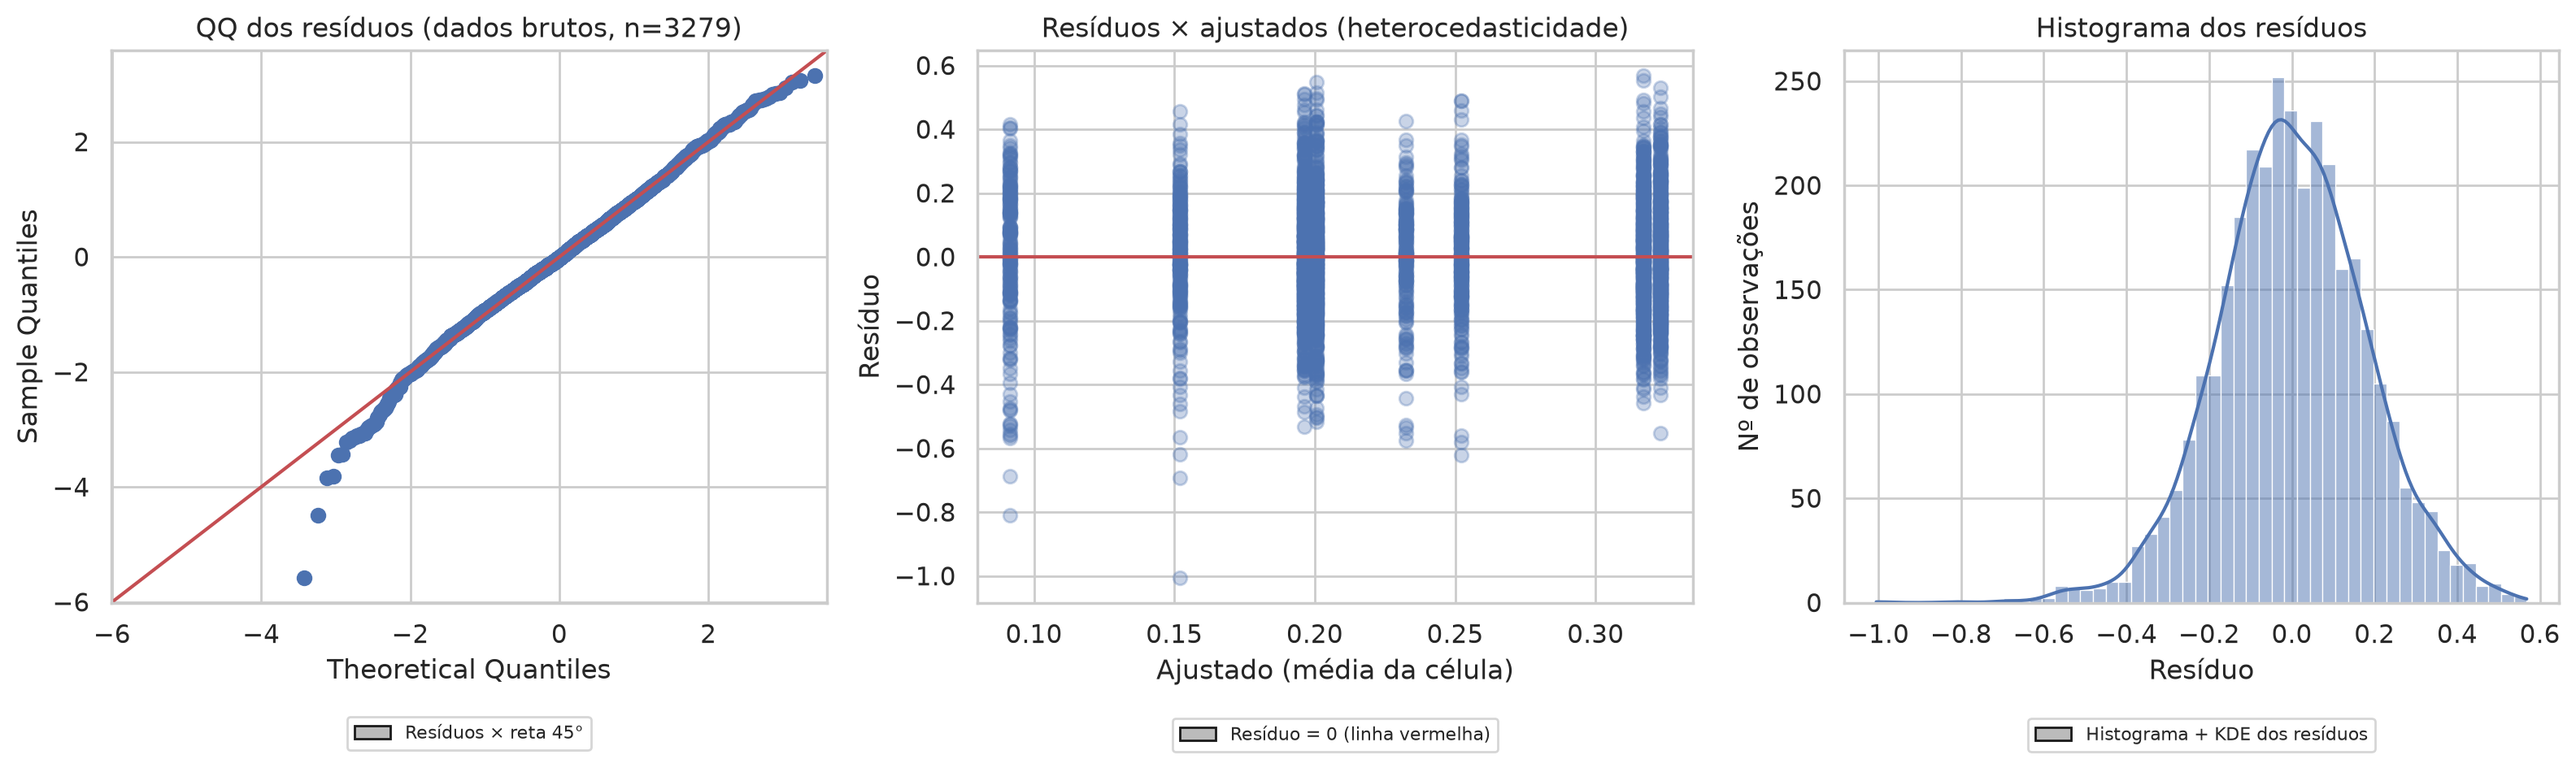
\includegraphics[width=\textwidth]{04_diagnostico_residuos.png}
\caption{Diagn\'ostico dos res\'iduos do modelo bruto ($n=3.279$): normalidade (QQ), res\'iduos $\times$ ajustados e histograma.}\label{fig:resid}
\end{figure}

%=====================================================================
\section{Caracteriza\c{c}\~ao e An\'alises Finais}
%=====================================================================
Interpretando os efeitos em unidades de GPA (m\'edia de $+$ menos m\'edia de $-$):
\begin{itemize}
\item \textbf{C (horas de estudo):} estudar acima da mediana acrescenta cerca de $0{,}121$ ponto em rela\c{c}\~ao a estudar at\'e a mediana; \'e o fator dominante (7,4\% da SQ total, contra 3,0\% de A).
\item \textbf{A (modo de uso):} o uso passivo reduz o \dgpa{} em cerca de $0{,}077$ em m\'edia (IC95\% $[-0{,}092;-0{,}062]$).
\item \textbf{AB:} a penaliza\c{c}\~ao do uso passivo \'e maior sob ansiedade alta: com pouco estudo, $-0{,}110$ (\emph{ab} $0{,}091$ vs.\ \emph{b} $0{,}201$) contra $-0{,}044$ com ansiedade baixa (\emph{a} $0{,}152$ vs.\ (1) $0{,}196$); com muito estudo, $-0{,}090$ contra $-0{,}065$. Isso sugere que a ansiedade amplifica o dano do uso passivo; a regress\~ao cont\'inua confirma a intera\c{c}\~ao.
\item \textbf{AC:} n\~ao significativa ($-0{,}0005$): a perda do uso passivo \'e semelhante com pouco estudo (m\'edia das duas ansiedades $-0{,}077$) e com muito estudo ($-0{,}078$).
\item \textbf{B:} efeito principal marginal e pequeno ($-0{,}0175$; IC exclui 0 por pouco; $p_{\text{HC3}}=0{,}027$; 0,15\% da SQ total).
\end{itemize}
Recomenda\c{c}\~ao pr\'atica preliminar: priorizar usos ativos da IA, especialmente em estudantes ansiosos; o ganho por estudar mais supera o de qualquer escolha de modo de uso.

%=====================================================================
\section{Discuss\~ao}
%=====================================================================
\textbf{Avalia\c{c}\~ao preliminar da hip\'otese.} Rejeita-se $H_0$ para A, C e AB (e, marginalmente, B), em consist\^encia com $H_1$: o uso passivo
reduz o \dgpa{} e o efeito depende da ansiedade. N\~ao h\'a evid\^encia de intera\c{c}\~ao com horas de estudo (AC, BC, ABC) nesta amostra.
O resultado \'e coerente com a Entrega 1 (ATE $=-0{,}072$), embora a PSM tenha mudado pouco o resultado porque as covari\'aveis j\'a estavam balanceadas ($|\text{SMD}|<0{,}05$).

\textbf{Limita\c{c}\~oes.}
\begin{itemize}
\item \emph{Pseudo-replica\c{c}\~ao:} as r\'eplicas bootstrap reusam os mesmos alunos e n\~ao s\~ao replica\c{c}\~ao experimental; por isso a ANOVA principal \'e ajustada aos 3.279 dados brutos com HC3, e o bootstrap serve apenas para os ICs.
\item \emph{Defini\c{c}\~ao de ``passivo'':} inclui \emph{Copywriting}, cujo \dgpa{} ($0{,}200$) \'e igual ao de \emph{Ideation}; o efeito vem quase todo de \emph{Direct Answer Generation} ($0{,}133$). Com a regra de extremos $Q_1/Q_3$, restringir a esse uso deixava as c\'elulas inviáveis ($n=17$--$31$); com a mediana essa an\'alise passa a ser poss\'ivel e est\'a prevista como pr\'oximo passo.
\item \emph{Teto de GPA 4,0:} afeta cerca de 12\% do recorte, gera assimetria nas c\'elulas passivas e pode subestimar ganhos.
\item \emph{Heterocedasticidade:} as c\'elulas passivas t\^em maior dispers\~ao (Levene $p<0{,}001$ nos dados brutos); tratada com ANOVA robusta (HC3) e IC bootstrap, que n\~ao assumem vari\^ancias iguais.
\item \emph{Dicotomiza\c{c}\~ao pela mediana:} perde informa\c{c}\~ao de vari\'aveis cont\'inuas ($R^2$ $0{,}129$ vs.\ $0{,}181$ no modelo cont\'inuo) e, na ansiedade (discreta), a mediana 4 deixa 53,4\% no n\'ivel baixo; por isso o efeito de B \'e pequeno e o contraste \'e ``acima vs.\ abaixo da mediana'', n\~ao ``muito vs.\ pouco''.
\item \emph{Dados observacionais:} n\~ao h\'a atribui\c{c}\~ao aleat\'oria do modo de uso; n\~ao se estabelece causalidade. A base provavelmente \'e sint\'etica, limitando a generaliza\c{c}\~ao.
\end{itemize}

\textbf{Mediana $\times$ quartis extremos.} A mediana usa 100\% do recorte (menor c\'elula 181 contra 36), reduz pela metade a largura dos ICs, evita exclus\~ao de alunos e tem regra simples e replic\'avel; por isso foi adotada como an\'alise principal. A regra de extremos produz efeitos maiores (C $+0{,}195$) por comparar grupos mais distantes, mas com poucos alunos e descartando 74\% dos dados. Ambas levam \`as mesmas conclus\~oes qualitativas.

\textbf{Corre\c{c}\~oes \`a Entrega 1.} A reavalia\c{c}\~ao dos dados mostrou que: a base tem 50.000 registros reais (n\~ao 10.000 simulados);
a tabela descritiva anterior estava incorreta (valores corretos na Tabela 1); a ansiedade n\~ao se concentra em 7--10 (moda $=4$);
e a narrativa de confus\~ao n\~ao era sustentada pelos dados.

%=====================================================================
\section{Conclus\~oes e Trabalhos Futuros}
%=====================================================================
O fatorial $2^3$ sobre os dados brutos, com erros robustos (HC3) e ICs por bootstrap estratificado, \'e vi\'avel com os n\'iveis definidos pela mediana (menor c\'elula $n=181$) e produz resultados est\'aveis entre sementes. As horas de estudo s\~ao o principal determinante do \dgpa{};
o uso passivo de IA reduz o \dgpa{} em cerca de $0{,}08$ e interage negativamente com a ansiedade alta. A heterocedasticidade das c\'elulas passivas \'e tratada por HC3 e IC bootstrap e permanece como limita\c{c}\~ao declarada.

\textbf{Ajustes planejados para a entrega final:}
\begin{itemize}
\item Citar a fonte e vers\~ao do conjunto de dados e documentar sua natureza.
\item Testar defini\c{c}\~oes alternativas de ``passivo'' (por exemplo, somente \emph{Direct Answer}) com c\'elulas maiores ou outros recortes.
\item Se necess\'ario, aprofundar o tratamento do teto de GPA (por exemplo, regress\~ao censurada), hoje apenas na an\'alise de sensibilidade (Ap\^endice~A).
\item Replicar em outros recortes (por exemplo, outras \'areas e anos) para avaliar generaliza\c{c}\~ao.
\end{itemize}

%=====================================================================
\appendix
\section{An\'alise de Sensibilidade e R\'eplicas Ilustrativas}
Este ap\^endice re\'une as t\'ecnicas complementares, que n\~ao entram na decis\~ao: normaliza\c{c}\~ao das m\'edias por bootstrap, ANOVA das r\'eplicas, estabilidade entre sementes, regras de corte alternativas, ANCOVA, regress\~ao cont\'inua, varredura de $m$, permuta\c{c}\~ao e tratamento do teto de GPA (reflex\~ao+raiz e regress\~ao quant\'ilica).

\subsection{Normaliza\c{c}\~ao das m\'edias pelo bootstrap (ilustrativo)}
Os dados brutos das c\'elulas passivas s\~ao assim\'etricos (com $n$ grande, o Shapiro--Wilk rejeita normalidade em 5 das 8 c\'elulas); as m\'edias bootstrap tornam-se normais
($p\ge0{,}077$ em todas as c\'elulas). As Figuras~\ref{fig:qq}, \ref{fig:histboot} e~\ref{fig:cdfboot} ilustram a normaliza\c{c}\~ao.

\begin{table}[H]
\centering
\caption{Assimetria e Shapiro--Wilk por c\'elula (bruto vs.\ m\'edias bootstrap).}
\begin{tabular}{crcccc}
\toprule
C\'elula & $n$ & Assim.\ bruta & $p$ bruto & Assim.\ boot. & $p$ boot.\\
\midrule
1 & 667 & 0,224 & 0,012 & $-0,125$ & 0,944\\
2 & 210 & $-1,127$ & $<0{,}001$ & 0,239 & 0,593\\
3 & 576 & 0,056 & 0,224 & 0,288 & 0,726\\
4 & 187 & $-0,798$ & $<0{,}001$ & 0,343 & 0,464\\
5 & 639 & 0,167 & 0,350 & 0,355 & 0,509\\
6 & 235 & $-0,299$ & 0,008 & 0,704 & 0,077\\
7 & 584 & 0,259 & 0,021 & $-0,145$ & 0,371\\
8 & 181 & $-0,719$ & $<0{,}001$ & 0,200 & 0,854\\
\bottomrule
\end{tabular}
\end{table}

\begin{figure}[H]\centering
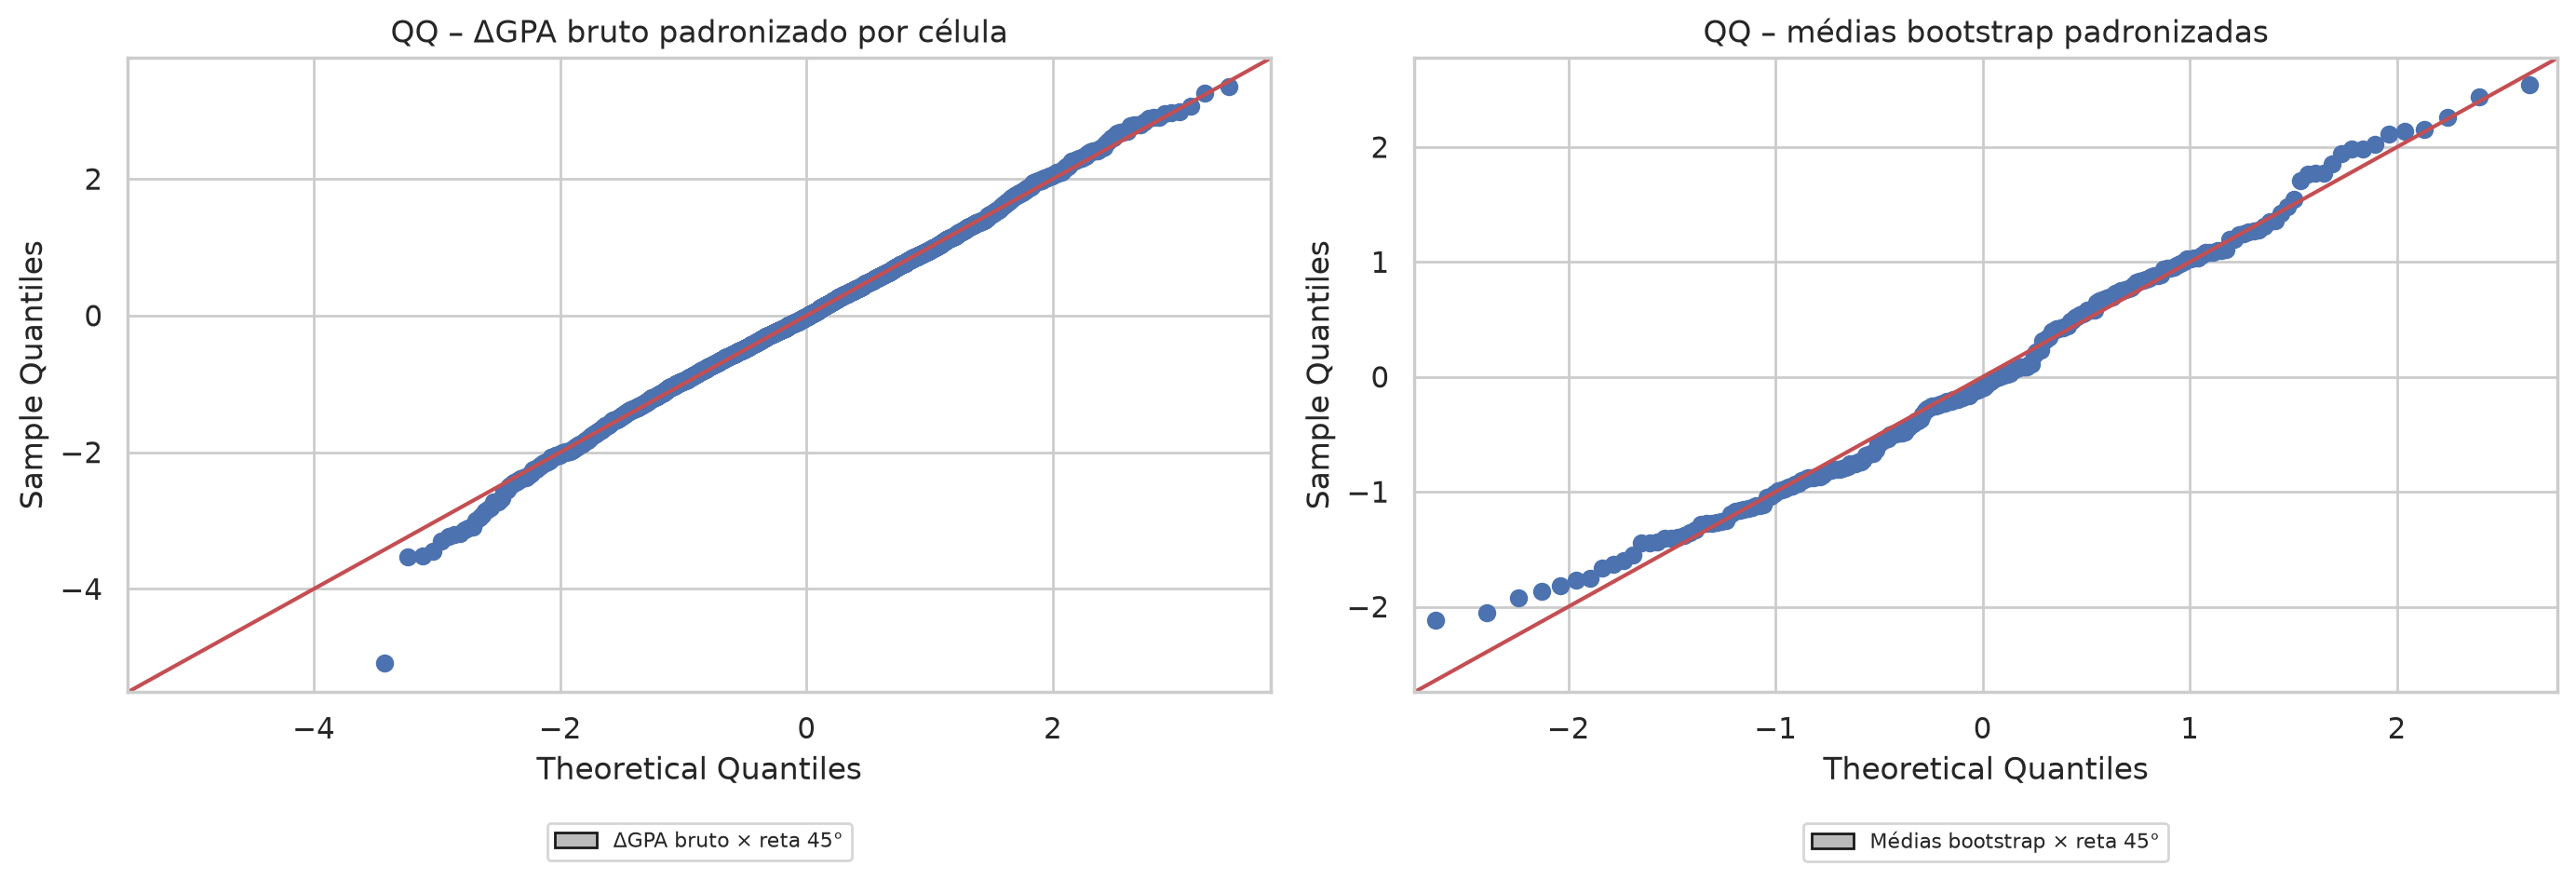
\includegraphics[width=\textwidth]{05_qq_antes_depois.png}
\caption{Gr\'aficos Q-Q antes (dados brutos) e depois (m\'edias bootstrap).}\label{fig:qq}
\end{figure}

\begin{figure}[H]\centering
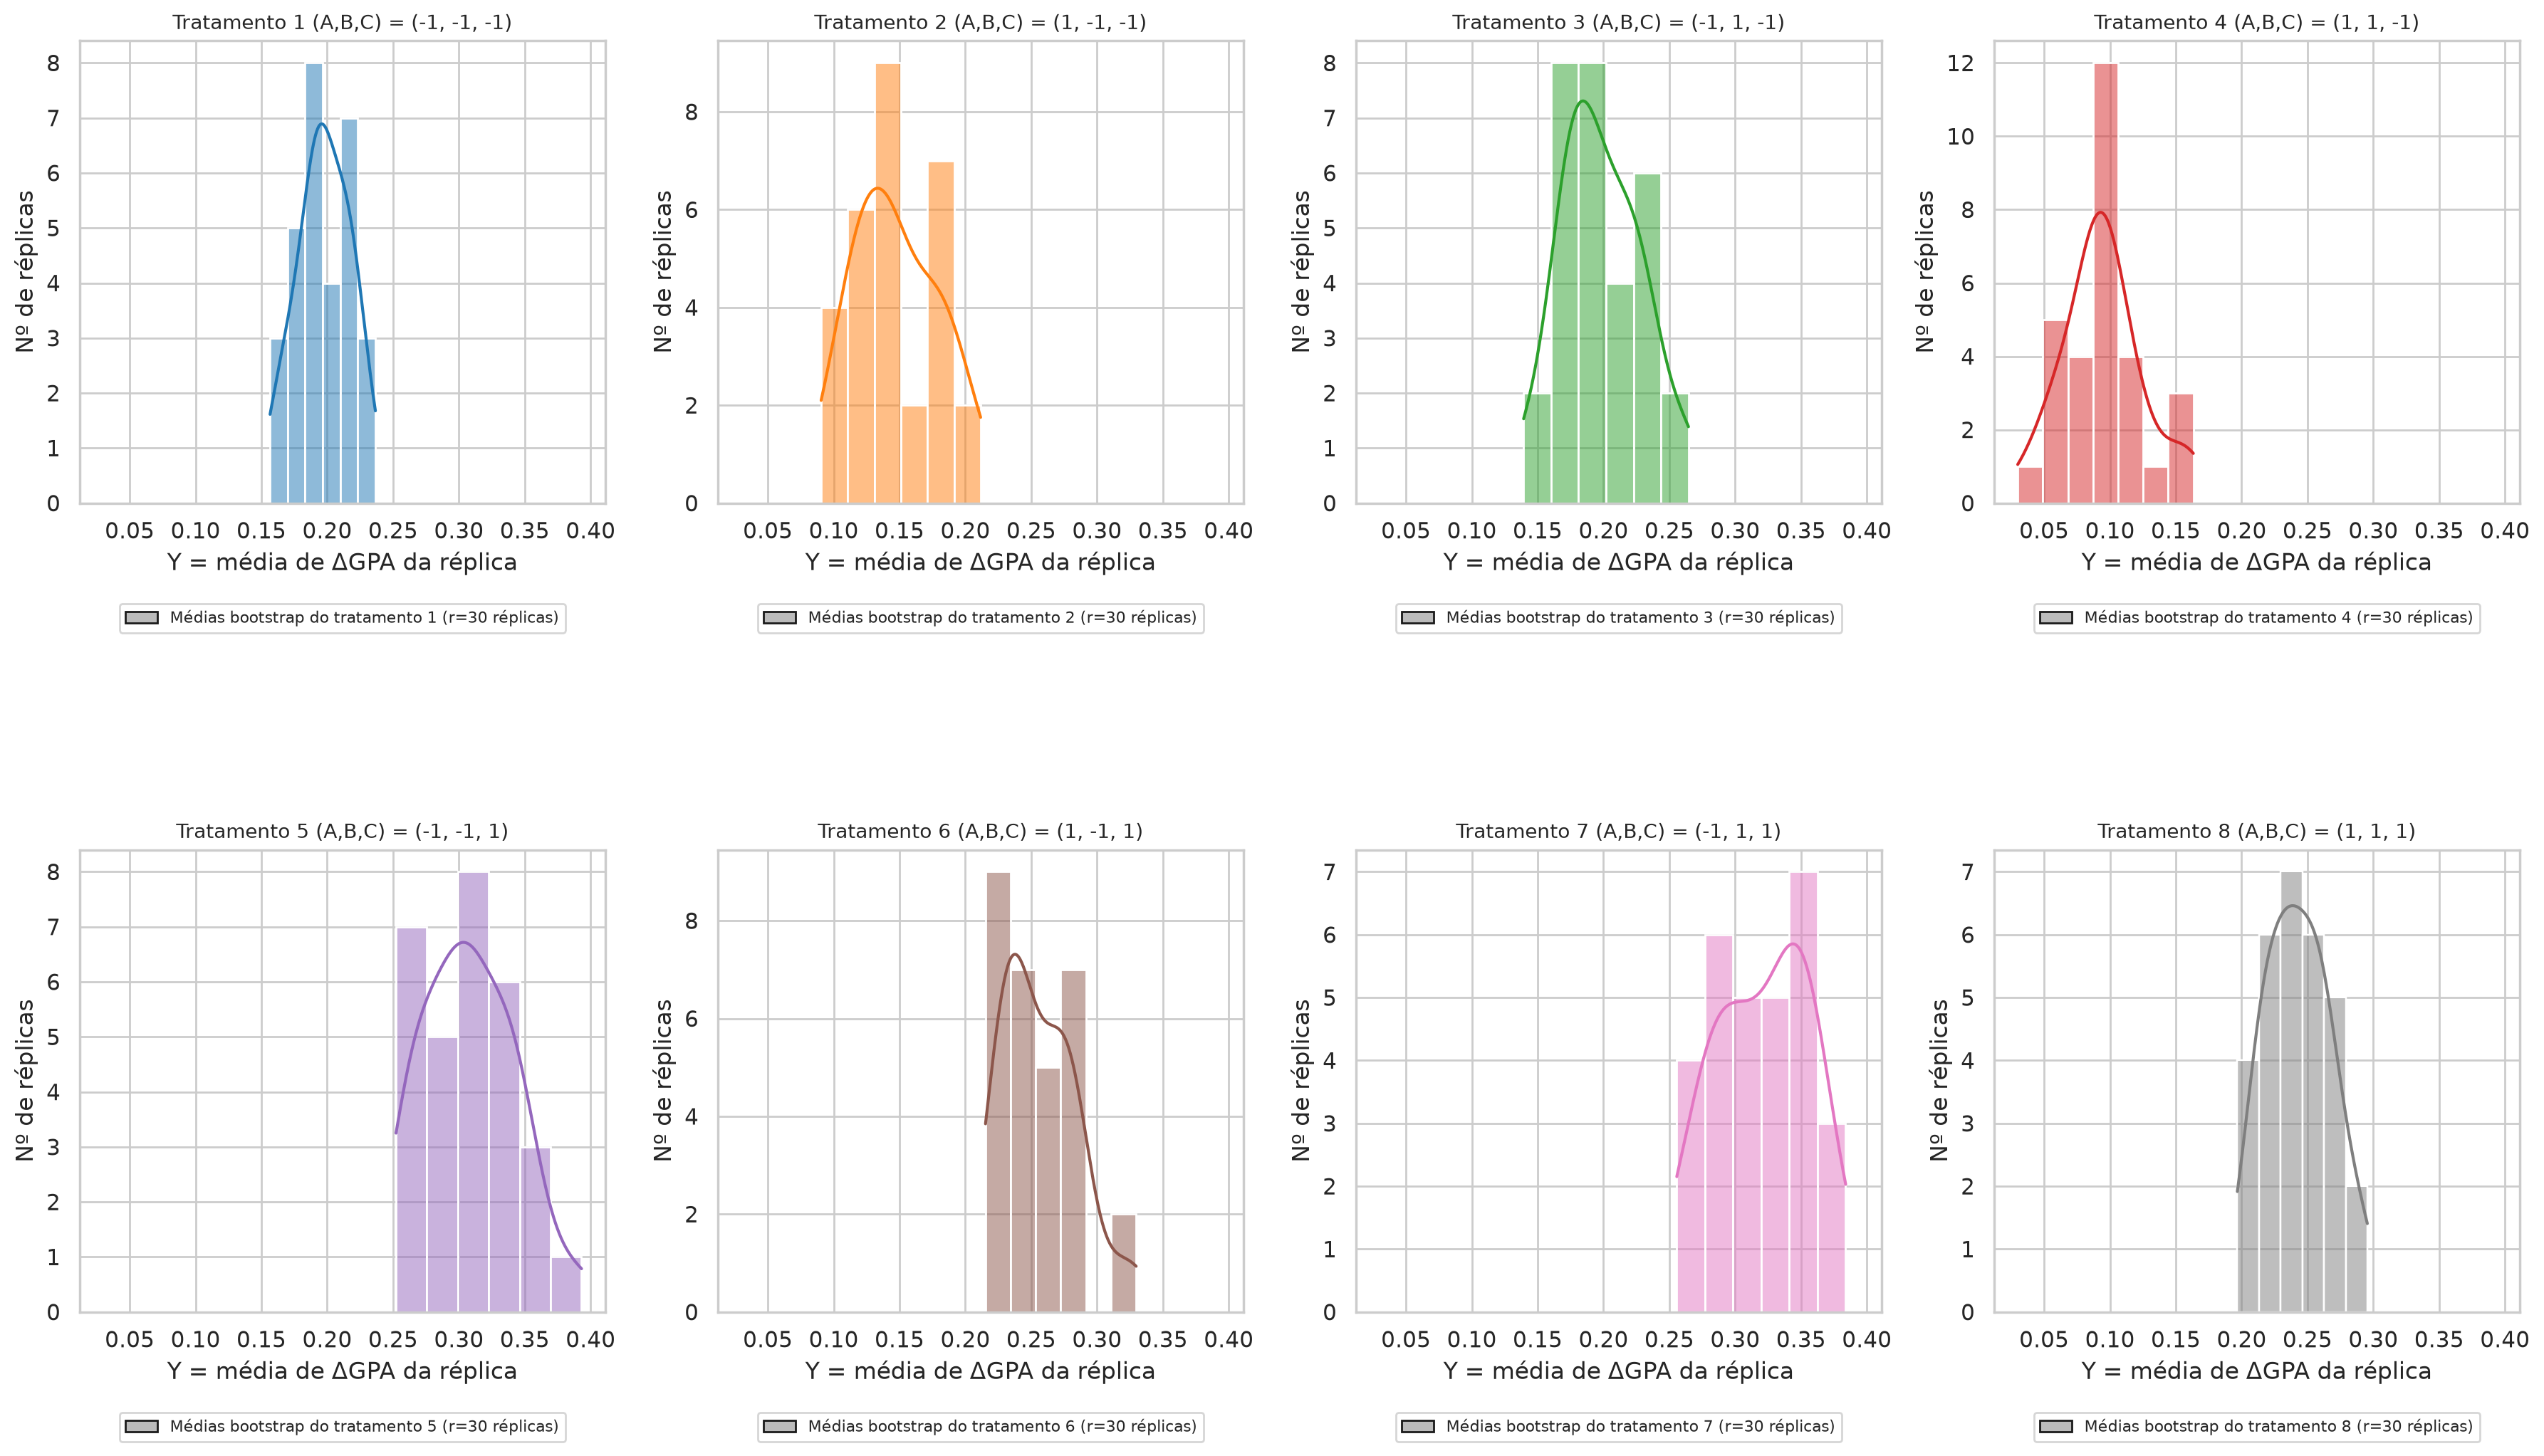
\includegraphics[width=\textwidth]{06_hist_bootstrap_por_celula.png}
\caption{Histogramas das m\'edias bootstrap por c\'elula.}\label{fig:histboot}
\end{figure}

\begin{figure}[H]\centering
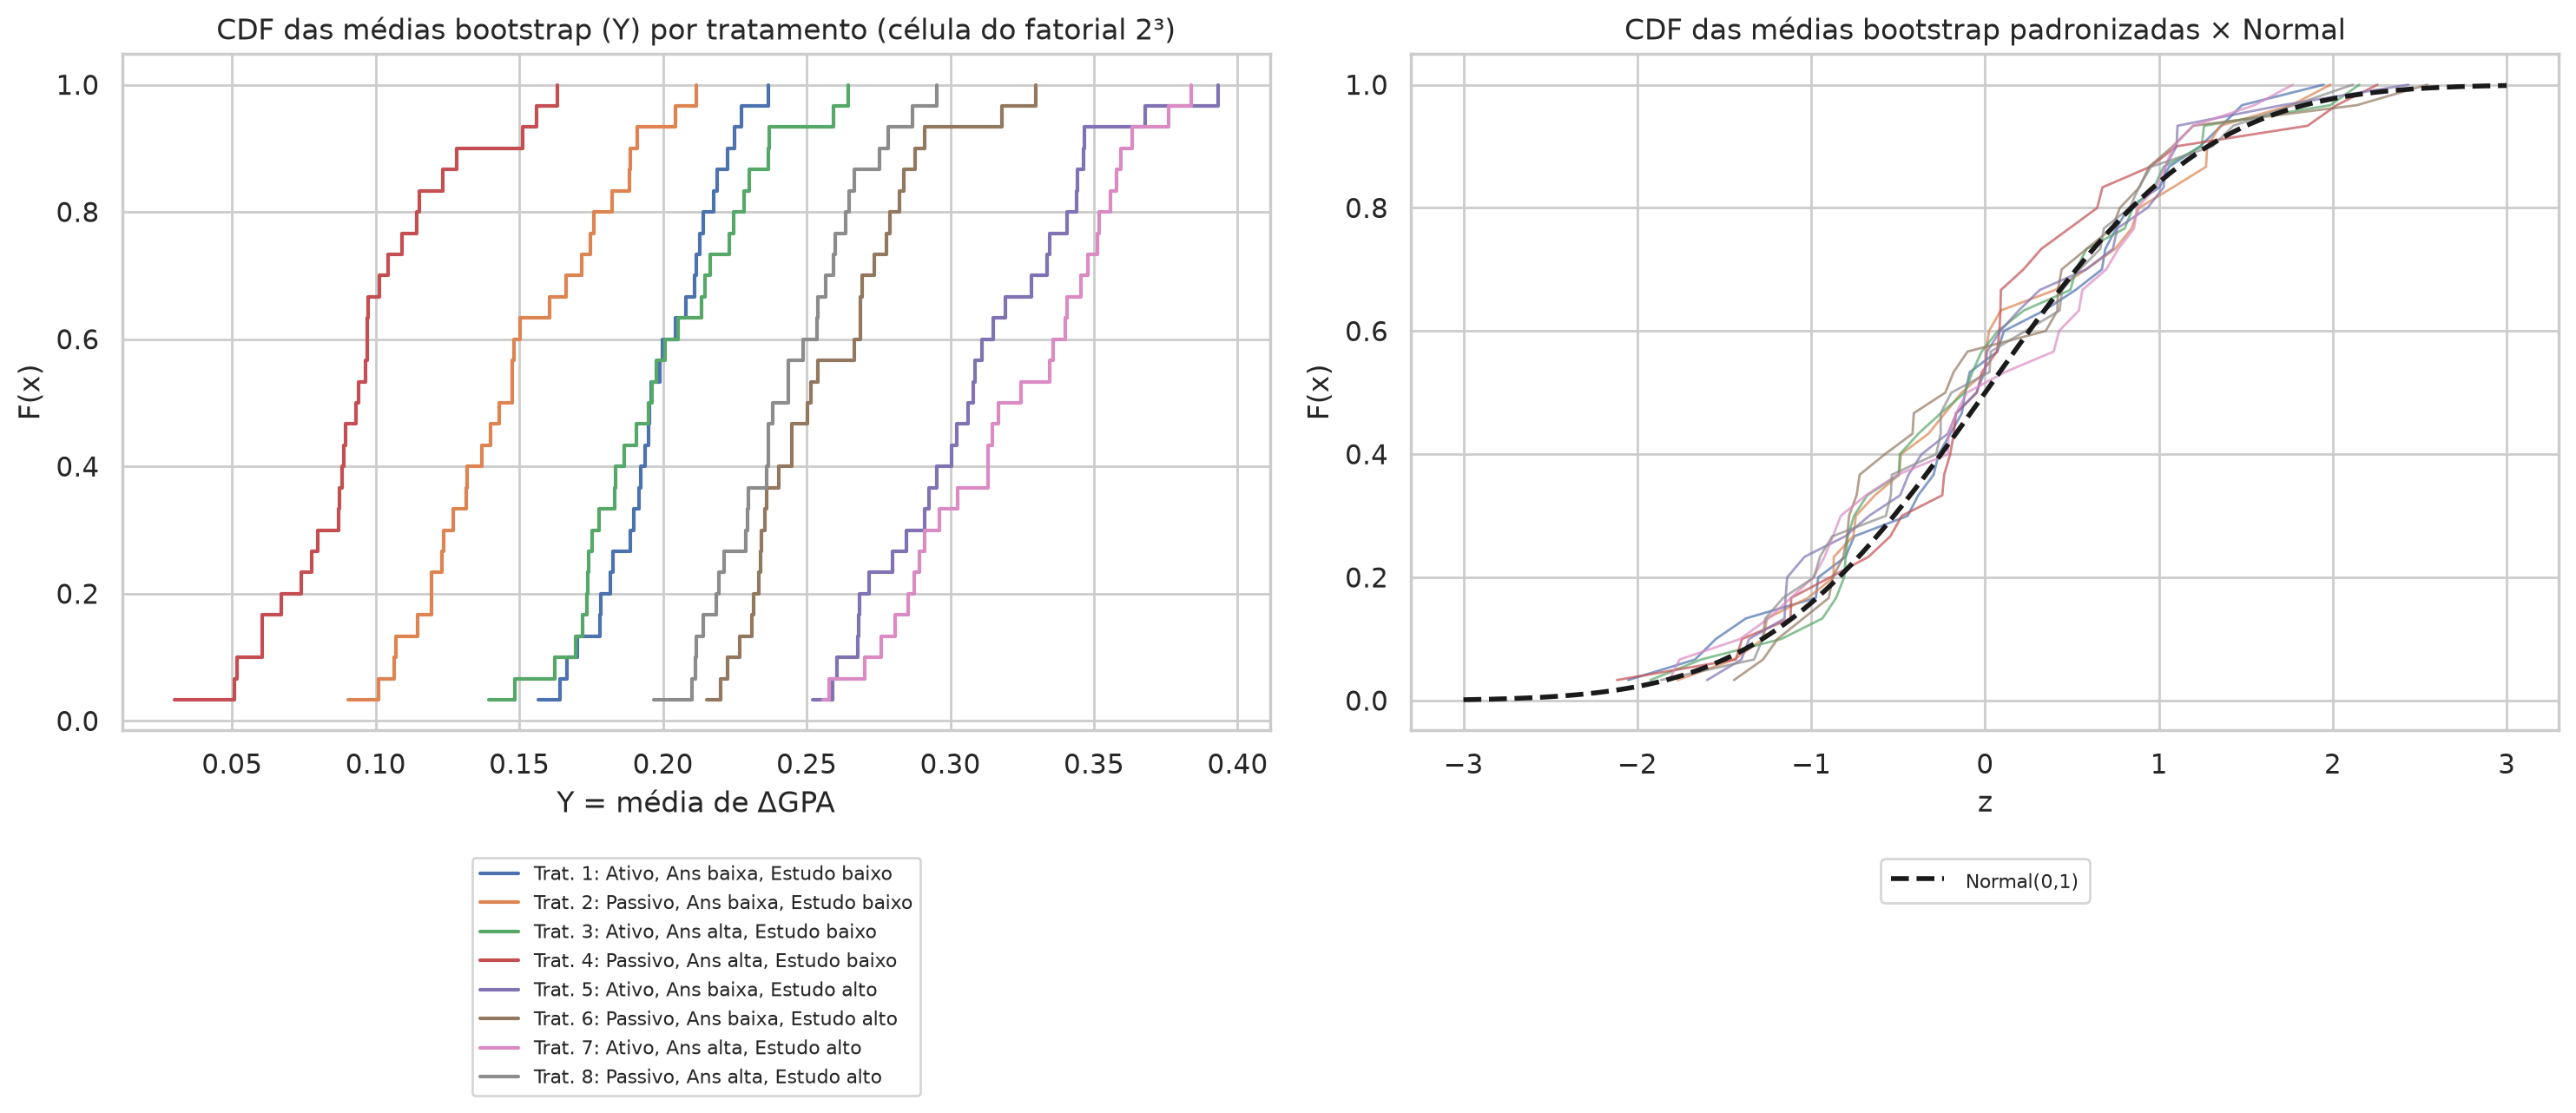
\includegraphics[width=\textwidth]{18_cdf_bootstrap.png}
\caption{CDF das m\'edias bootstrap versus CDF normal te\'orica.}\label{fig:cdfboot}
\end{figure}

\subsection{ANOVA sobre as r\'eplicas bootstrap (descritiva)}
\begin{table}[H]
\centering
\caption{ANOVA sobre as 240 observa\c{c}\~oes bootstrap.}
\begin{tabular}{lrrrrr}
\toprule
Fonte & SQ & GL & $F$ & $p$ & \% var.\\
\midrule
A & 0,3005 & 1 & 331,6 & $<0{,}001$ & 20,6\\
B & 0,0107 & 1 & 11,8 & $<0{,}001$ & 0,7\\
C & 0,9016 & 1 & 994,8 & $<0{,}001$ & 61,7\\
AB & 0,0241 & 1 & 26,5 & $<0{,}001$ & 1,6\\
AC & 0,0024 & 1 & 2,6 & 0,108 & 0,2\\
BC & 0,0097 & 1 & 10,8 & 0,001 & 0,7\\
ABC & 0,0028 & 1 & 3,1 & 0,078 & 0,2\\
Res\'iduo & 0,2103 & 232 & -- & -- & 14,4\\
\bottomrule
\end{tabular}
\end{table}

\textbf{Aten\c{c}\~ao:} os $p$-valores desta ANOVA s\~ao otimistas (at\'e BC, nulo, aparece com $p=0{,}001$), pois as r\'eplicas reutilizam os mesmos alunos.
Por isso ela \emph{n\~ao} \'e usada na decis\~ao (a infer\^encia \'e feita pelo modelo bruto com HC3 e pelo IC bootstrap), e o \% de vari\^ancia desta tabela (C $=61{,}7\%$) \'e inflado pela remo\c{c}\~ao da variabilidade entre alunos.

\subsection{Diagn\'ostico dos res\'iduos das r\'eplicas}
Nas r\'eplicas, o Shapiro--Wilk dos res\'iduos d\'a $p=0{,}115$ (normalidade aceita) e o Levene $p=0{,}044$ (no limiar), reflexo da maior dispers\~ao das c\'elulas passivas.
\begin{figure}[H]\centering
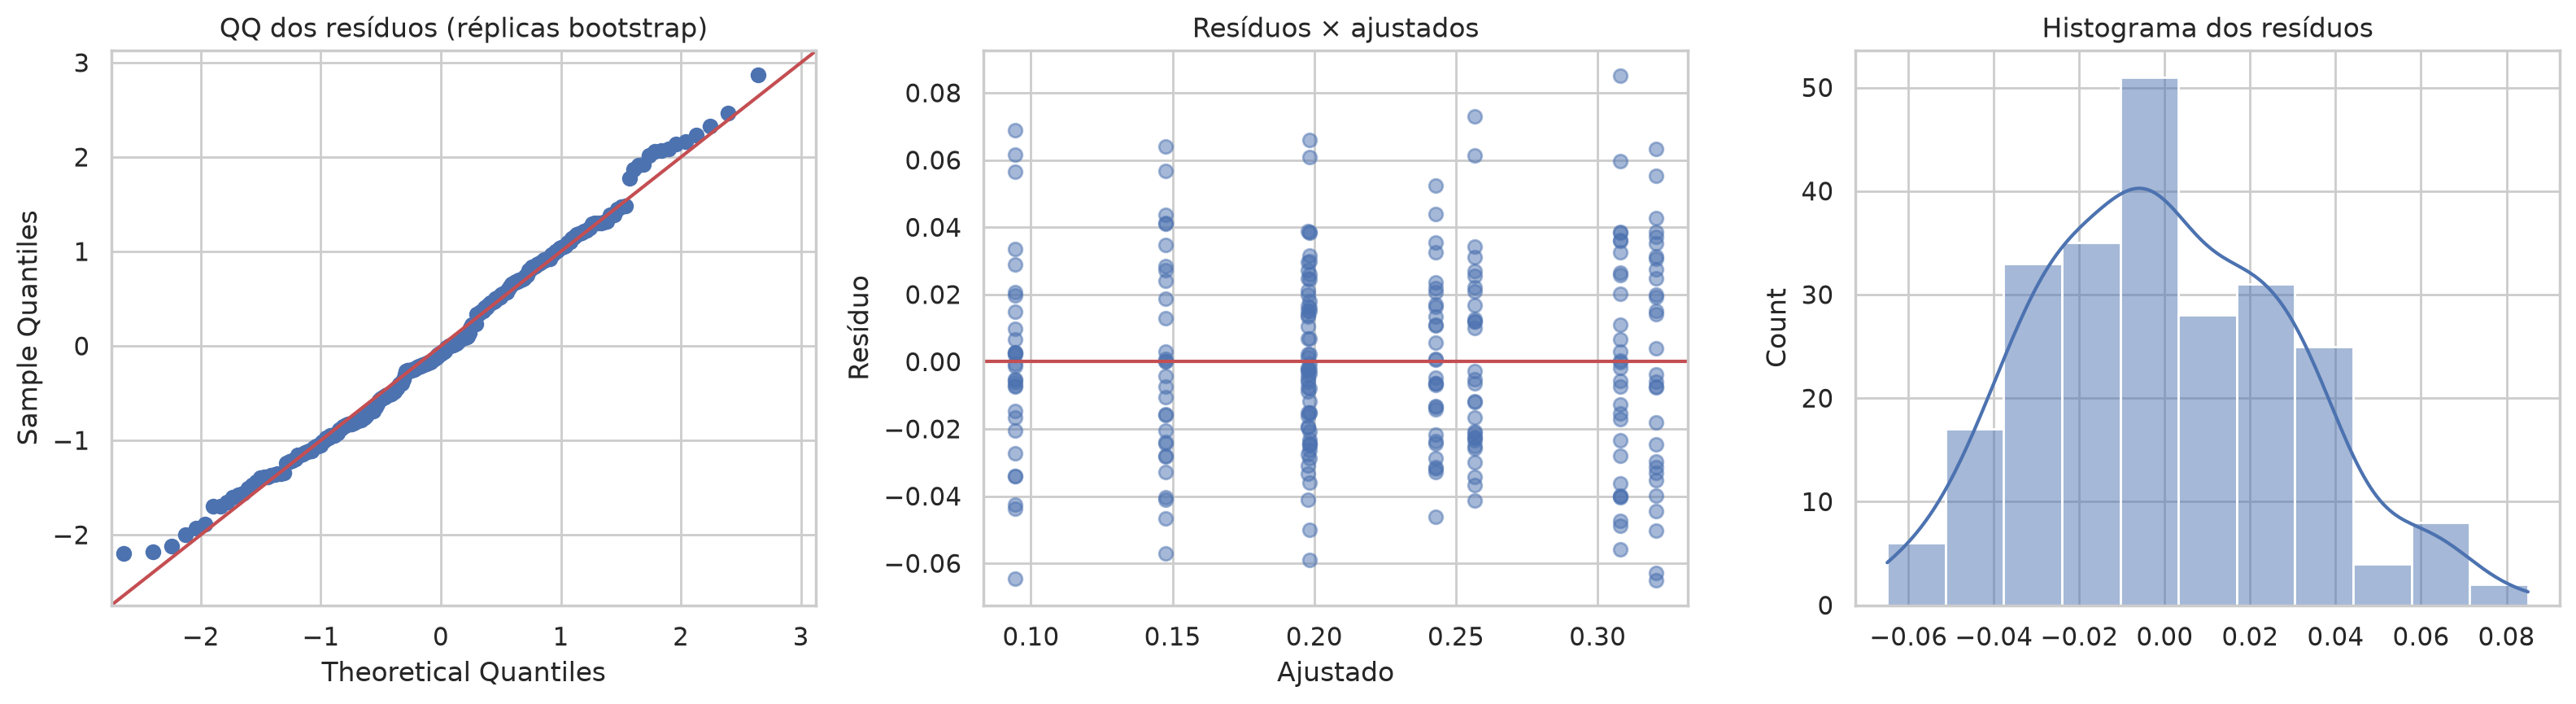
\includegraphics[width=\textwidth]{04b_diagnostico_residuos_replicas.png}
\caption{Diagn\'ostico dos res\'iduos da ANOVA das r\'eplicas bootstrap.}\label{fig:residrep}
\end{figure}

\subsection{Estabilidade entre sementes}
Repetindo o procedimento com 10 sementes, o desvio-padr\~ao dos efeitos fica entre $0{,}0027$ e $0{,}0056$
(A: $-0{,}0772\pm0{,}0056$; C: $+0{,}1228\pm0{,}0029$; AB: $-0{,}0220\pm0{,}0027$), de modo que as conclus\~oes n\~ao dependem da semente.

\subsection{Sensibilidade \`a defini\c{c}\~ao dos n\'iveis, ANCOVA e regress\~ao cont\'inua}
\begin{table}[H]
\centering
\caption{Efeitos sob defini\c{c}\~oes alternativas de n\'ivel (* = IC95\% exclui 0).}
\small\setlength{\tabcolsep}{3pt}
\begin{tabular}{lrrrrrrrr}
\toprule
Defini\c{c}\~ao & $n$ & A & B & C & AB & AC & BC & ABC\\
\midrule
Mediana (principal) & 3.279 & $-0{,}077^*$ & $-0{,}017^*$ & $+0{,}121^*$ & $-0{,}023^*$ & $0{,}000$ & $+0{,}011$ & $+0{,}010$\\
$<Q_1/\ge Q_3$ (vers\~ao anterior) & 848 & $-0{,}067^*$ & $-0{,}043^*$ & $+0{,}195^*$ & $-0{,}046^*$ & $+0{,}022$ & $+0{,}004$ & $-0{,}006$\\
$\le Q_1/\ge Q_3$ & 1.101 & $-0{,}080^*$ & $-0{,}038^*$ & $+0{,}193^*$ & $-0{,}033^*$ & $+0{,}011$ & $+0{,}006$ & $+0{,}005$\\
\bottomrule
\end{tabular}
\end{table}
Os sinais, a signific\^ancia de A, C e AB e a ordem de import\^ancia se mant\^em nas tr\^es regras; mudam as magnitudes de B, C e AB, que caem cerca de 40--50\% com a mediana porque o contraste deixa de ser ``extremo $\times$ extremo'' e passa a ``acima $\times$ abaixo da mediana''.
Uma ANCOVA com \texttt{Pre\_GPA} como covari\'avel d\'a A $=-0{,}076$, B $=-0{,}018$, C $=+0{,}121$ e AB $=-0{,}022$, praticamente id\^enticos aos principais.
Uma regress\~ao cont\'inua (sem dicotomizar B e C; $R^2=0{,}181$, contra $0{,}129$ do modelo dicotomizado) confirma: cada hora de estudo adiciona $+0{,}014$ ($p<0{,}001$), cada ponto de ansiedade reduz $0{,}005$ ($p=0{,}002$) e a intera\c{c}\~ao uso passivo $\times$ ansiedade \'e $-0{,}0064$ por ponto ($p<0{,}001$).

\begin{figure}[H]\centering
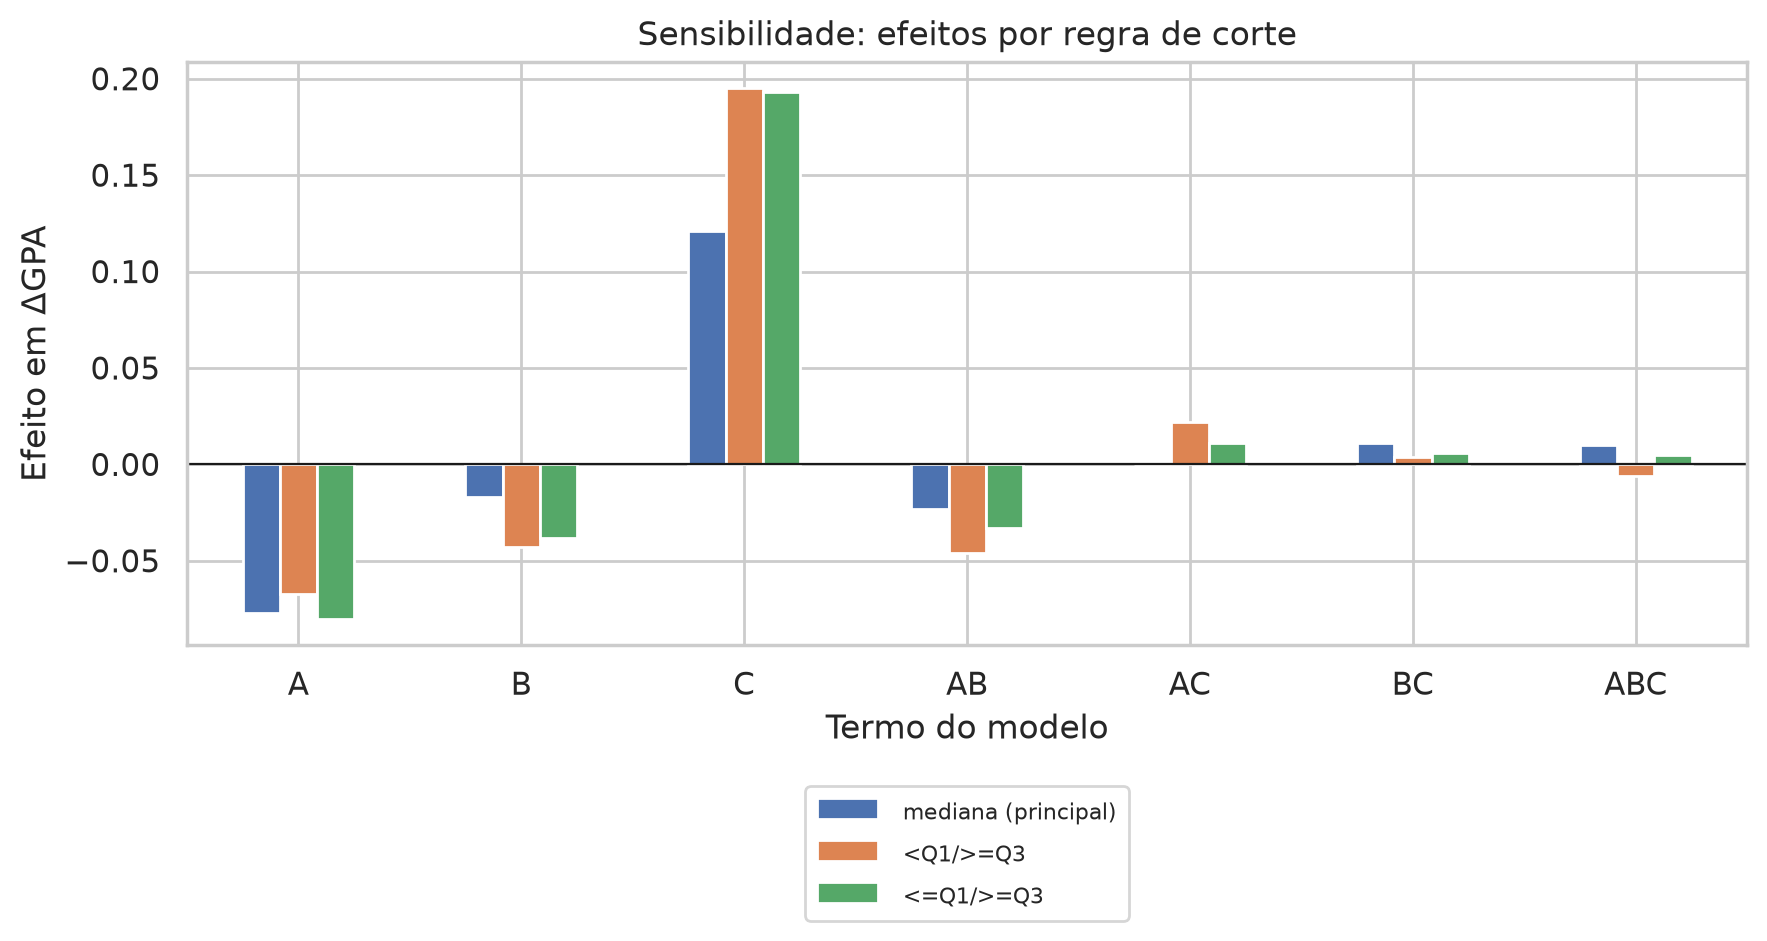
\includegraphics[width=\textwidth]{14_sensibilidade.png}
\caption{Sensibilidade dos efeitos \`a defini\c{c}\~ao dos n\'iveis.}\label{fig:sens}
\end{figure}

\subsection{Balanceamento, permuta\c{c}\~ao e teto de GPA}
O desbalanceamento ($n=181$--$667$) n\~ao enviesa as estimativas, mas elimina a ortogonalidade dos contrastes e torna desigual a precis\~ao por c\'elula; a amostragem com $m$ igual por c\'elula restaura o balanceamento. O bootstrap, entretanto, \emph{n\~ao normaliza} o $\Delta$GPA bruto (assimetria por causa do teto 4,0): apenas aproxima a distribui\c{c}\~ao das m\'edias. A Tabela~\ref{tab:esquemas} compara esquemas de r\'eplica ($r=300$).
\begin{table}[H]\centering\small
\begin{tabular}{lccc}\toprule
Esquema & $A$ & $C$ & $AB$\\\midrule
bootstrap $m=36$ (atual) & $-0{,}075$ & $+0{,}121$ & $-0{,}023$\\
bootstrap $m=150$ & $-0{,}077$ & $+0{,}121$ & $-0{,}023$\\
sem reposi\c{c}\~ao $m=150$ & $-0{,}078$ & $+0{,}121$ & $-0{,}023$\\
sem reposi\c{c}\~ao $m=181$ & $-0{,}077$ & $+0{,}121$ & $-0{,}023$\\\bottomrule
\end{tabular}\caption{Efeitos m\'edios por esquema de r\'eplica.}\label{tab:esquemas}
\end{table}
Os efeitos s\~ao id\^enticos ($\pm0{,}003$): a estimativa n\~ao depende de $m$ nem da reposi\c{c}\~ao (Fig.~\ref{fig:varm}). O desvio-padr\~ao entre r\'eplicas sem reposi\c{c}\~ao diminui com $m$ por efeito de popula\c{c}\~ao finita ($\approx0{,}021$ em $m=36$ e $\approx0{,}006$ em $m=181$) e n\~ao representa o erro do estimador; por isso Shapiro e Levene das r\'eplicas sem reposi\c{c}\~ao falham por constru\c{c}\~ao, e o IC de infer\^encia permanece o do bootstrap completo.
\begin{figure}[H]\centering
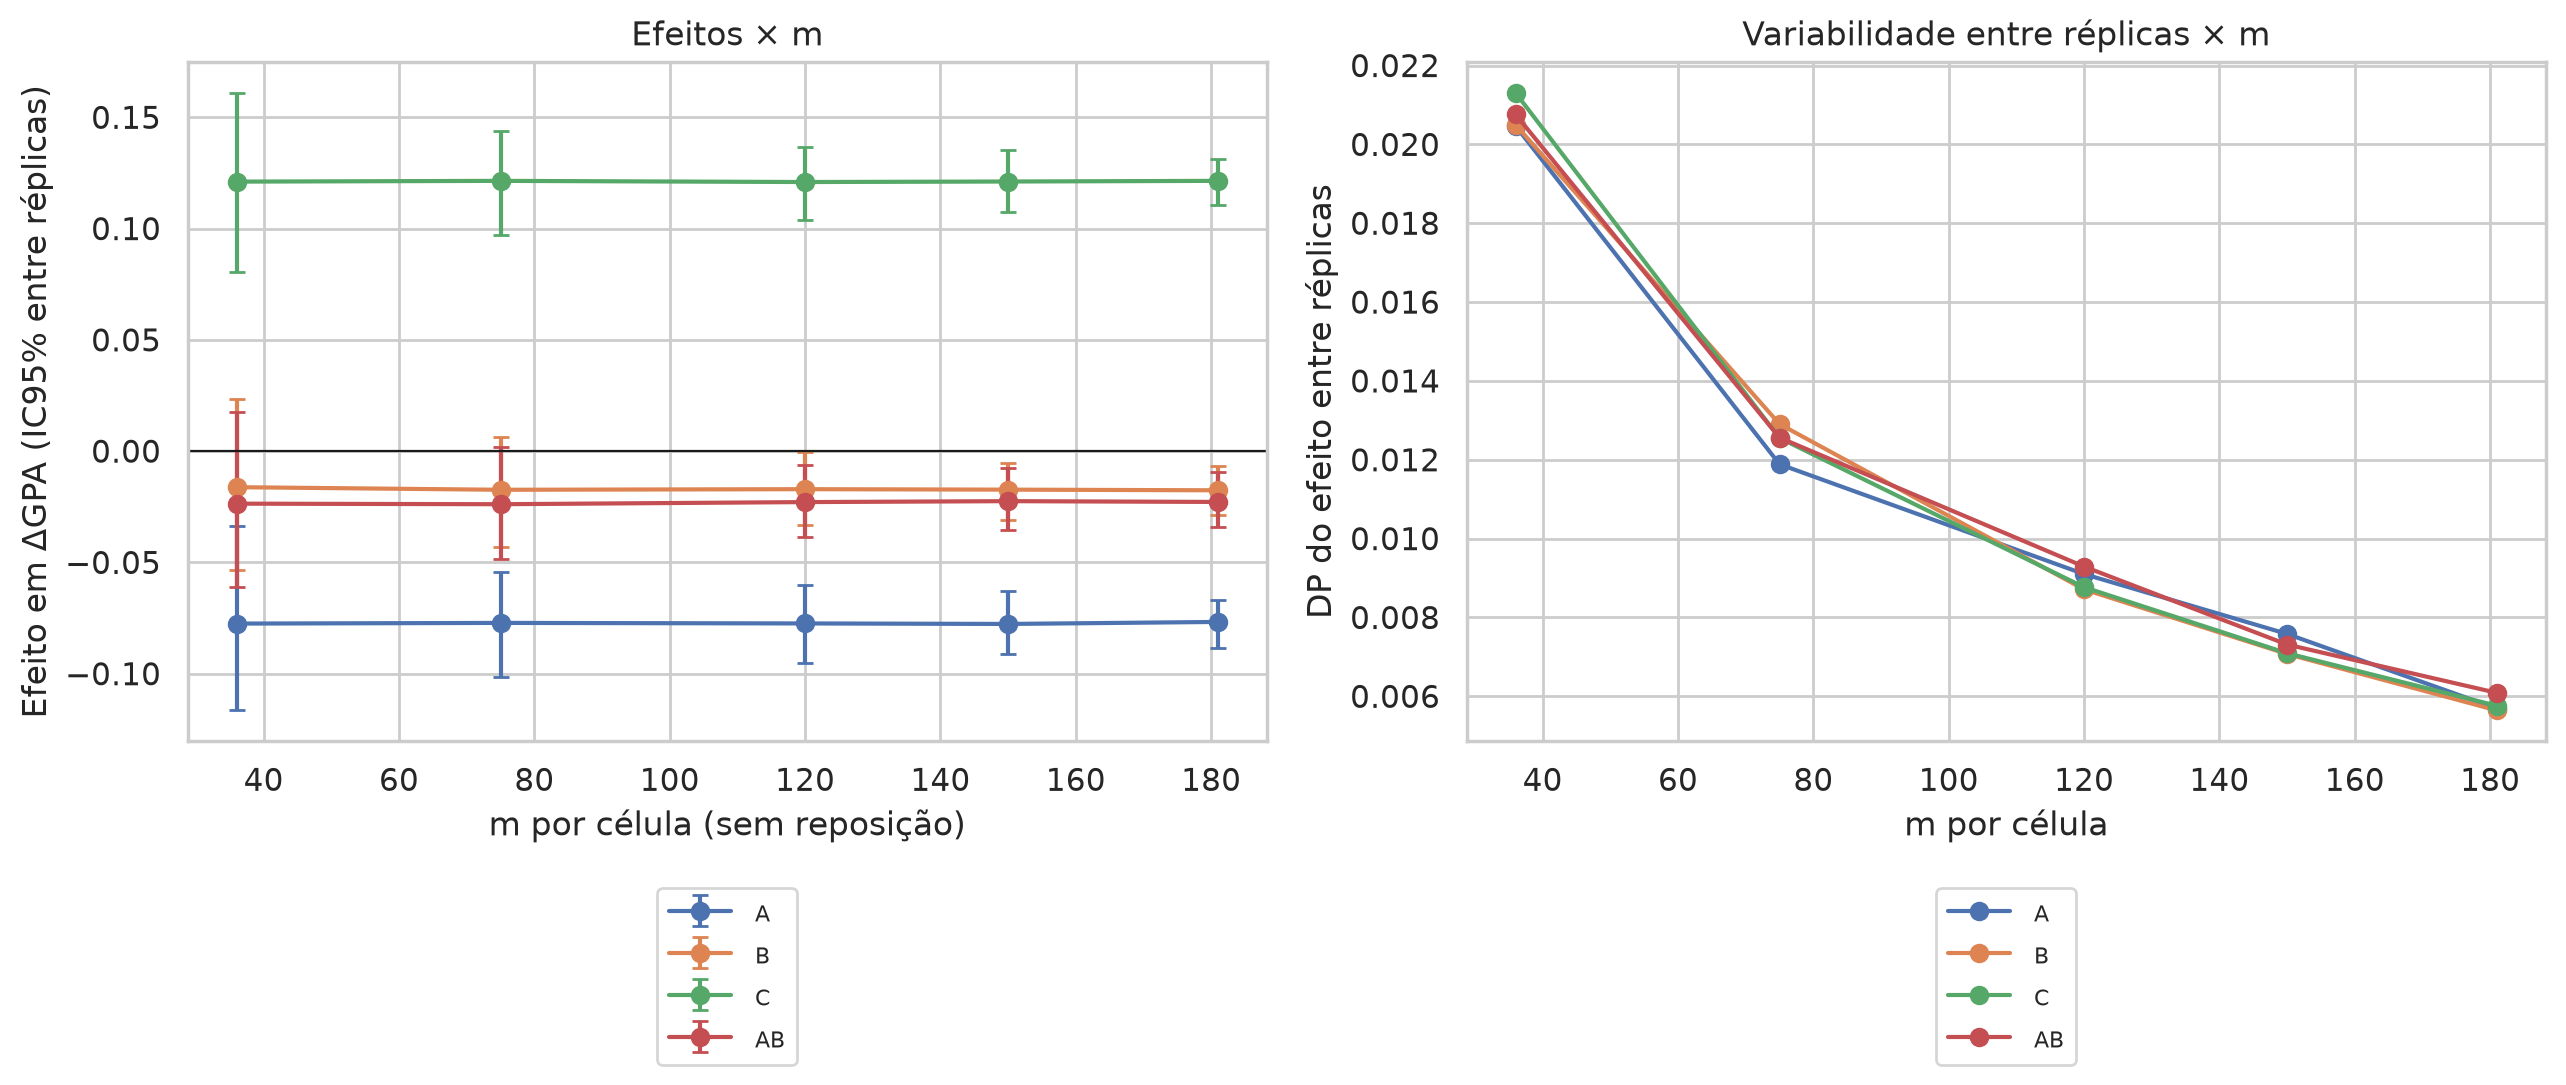
\includegraphics[width=\textwidth]{20_varredura_m.png}
\caption{Efeitos e variabilidade entre r\'eplicas em fun\c{c}\~ao de $m$ (sem reposi\c{c}\~ao).}\label{fig:varm}
\end{figure}
O teste de permuta\c{c}\~ao (5.000, res\'iduos do modelo reduzido) fornece $p=0{,}0002$ (A), $0{,}0002$ (C), $0{,}0016$ (AB), $0{,}95$ (AC), $0{,}145$ (BC) e $0{,}18$ (ABC), concordando com IC bootstrap e HC3. Para B, $p=0{,}019$, em linha com HC3 ($0{,}027$) e ANOVA bruta ($0{,}017$): efeito marginal e de magnitude desprez\'ivel ($0{,}15\%$ da SQ total). Com transforma\c{c}\~ao (reflex\~ao + raiz) e regress\~ao quant\'ilica para o teto de GPA (12,1\% no valor 4,0), os sinais se mant\^em (A $-0{,}051$, C $+0{,}114$ na mediana).
\begin{figure}[H]\centering
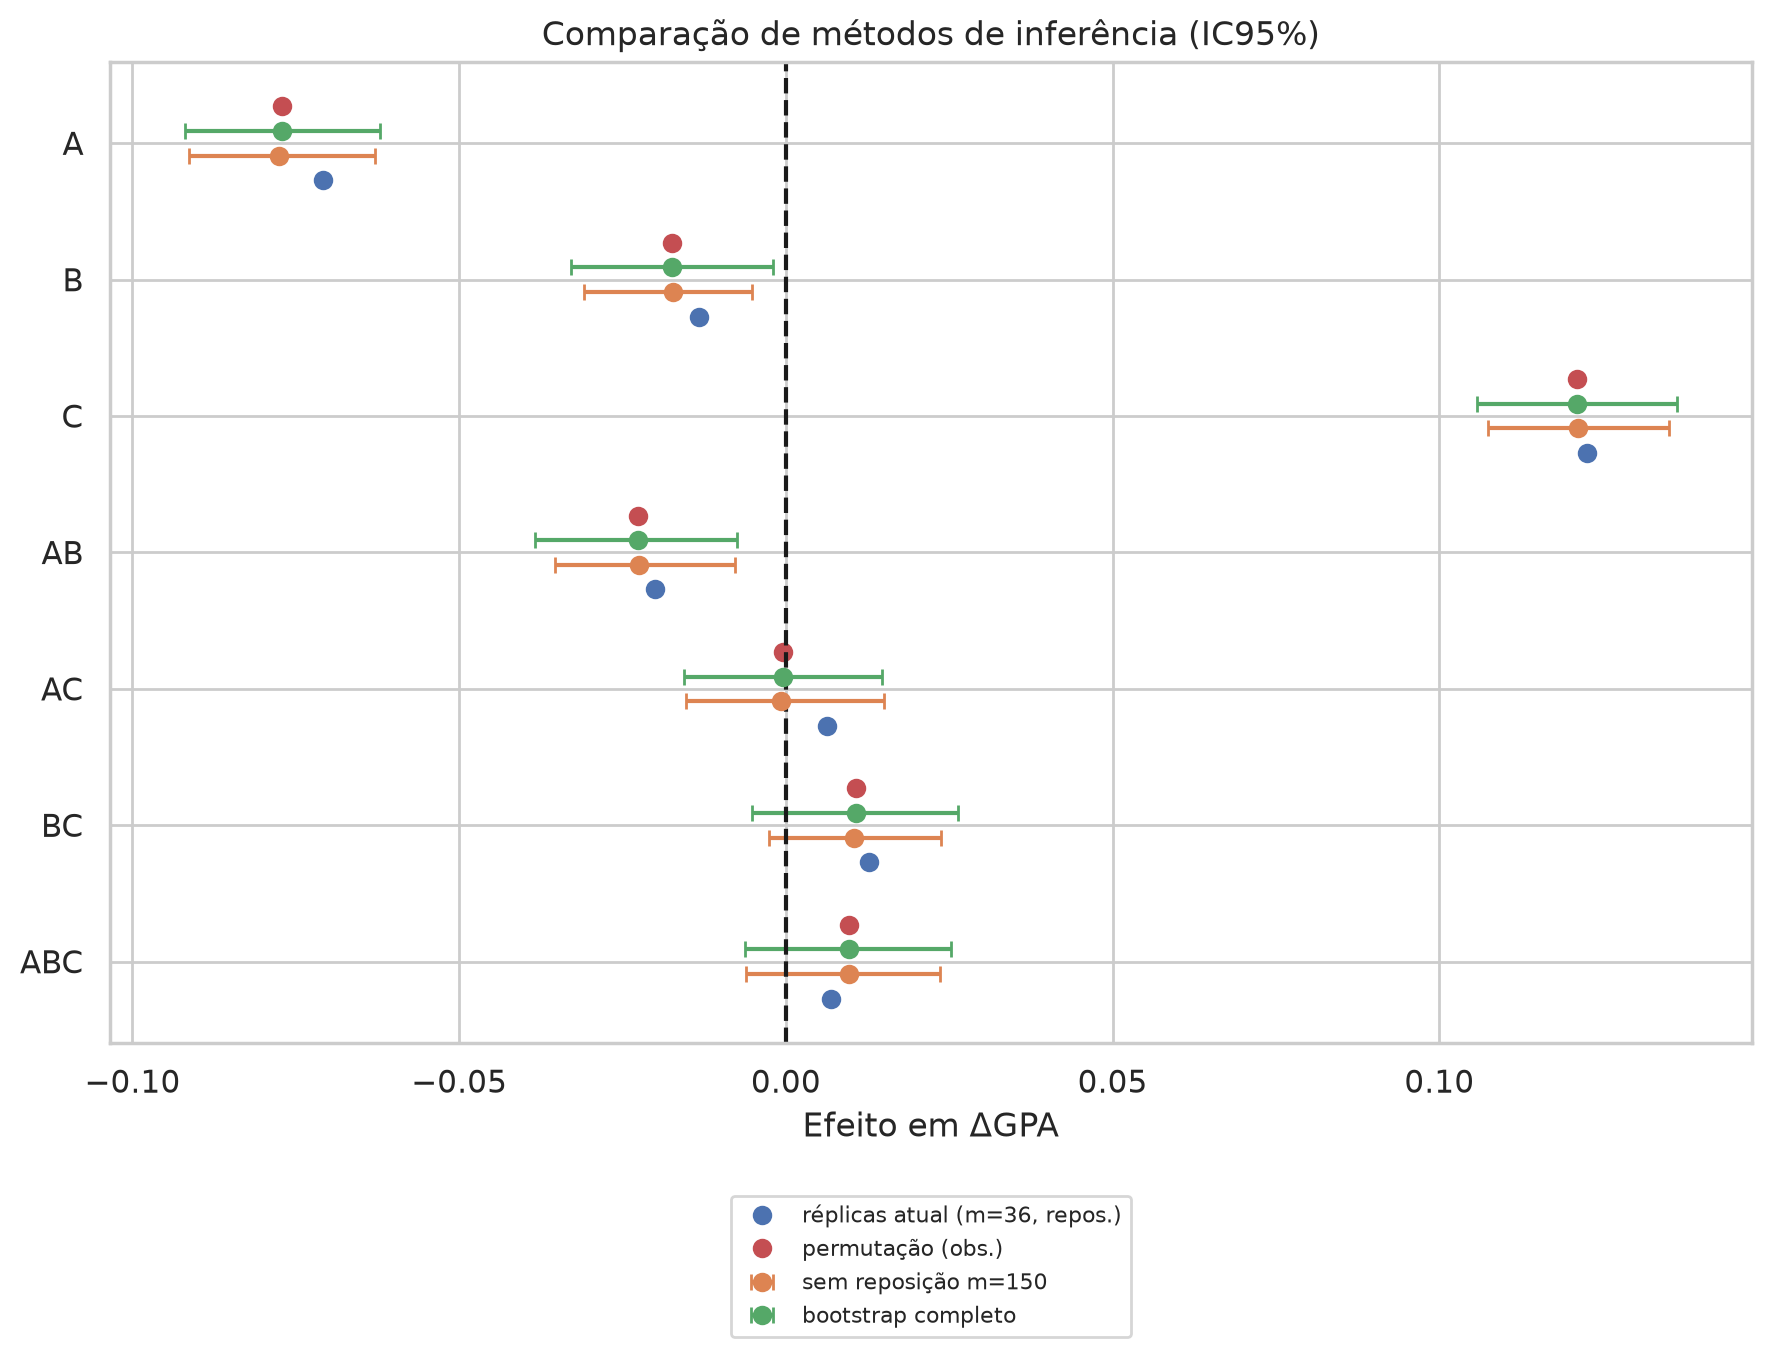
\includegraphics[width=.9\textwidth]{21_comparacao_metodos.png}
\caption{Efeitos e IC95\% por m\'etodo de infer\^encia.}\label{fig:metodos}
\end{figure}
\begin{figure}[H]\centering
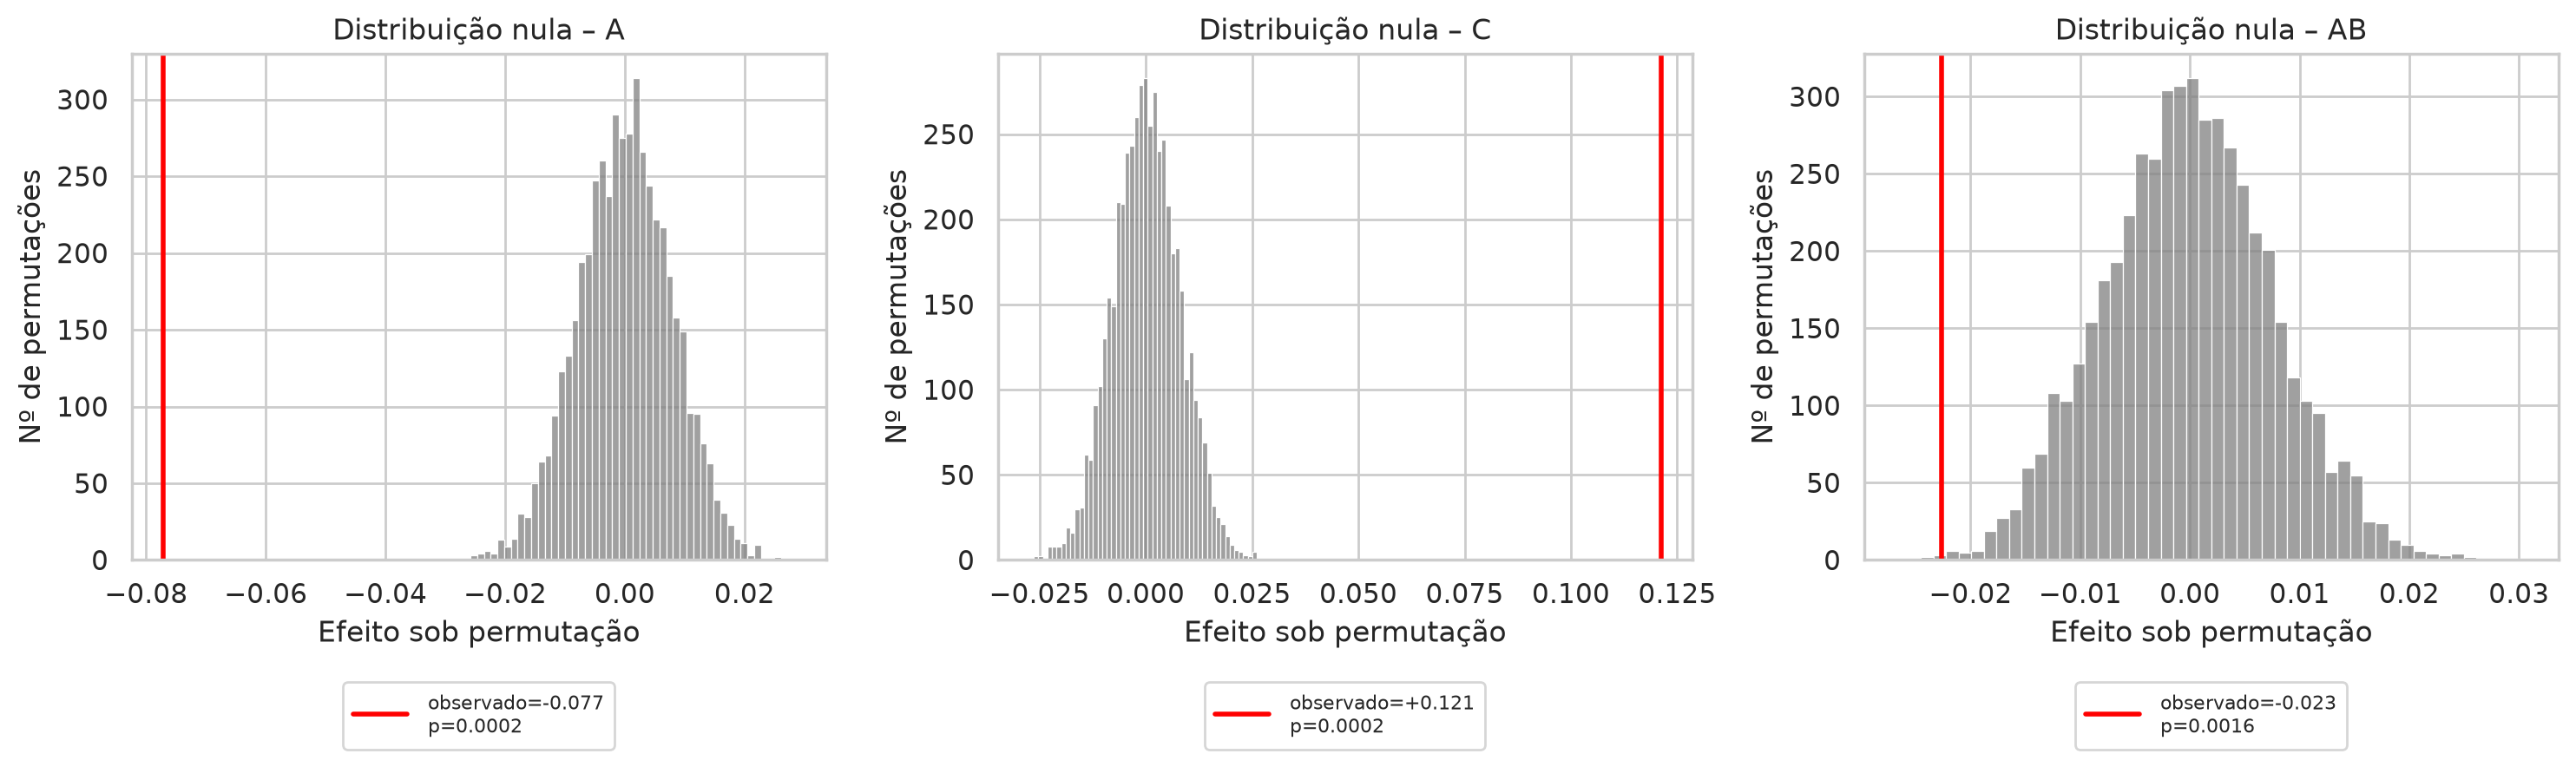
\includegraphics[width=\textwidth]{22_permutacao_nulo.png}
\caption{Distribui\c{c}\~ao nula da permuta\c{c}\~ao e efeito observado (A, C, AB).}\label{fig:perm}
\end{figure}
Conclus\~ao: os m\'etodos concordam; a an\'alise principal permanece o modelo bruto com HC3 e IC bootstrap, e as demais t\'ecnicas servem apenas de verifica\c{c}\~ao.

\section{Reprodutibilidade}
%=====================================================================
\begin{itemize}
\item Par\^ametros: \texttt{SEED}=42, $r=30$, $m=36$, \texttt{NBOOT}=5.000, \texttt{REGRA}=``mediana'' (``quartis'' reproduz a vers\~ao anterior, arquivada em \texttt{entrega2/dados/quartis/}).
\item C\'odigo: \texttt{entrega2/pcc170\_entrega02.py} (fonte \'unica) e \texttt{pcc170\_entrega02.ipynb}.
\item Figuras: \texttt{entrega2/figuras/} (24 arquivos + \texttt{separados/}); tabelas CSV: \texttt{entrega2/dados/}.
\item Dados: \texttt{csv/ai\_student\_impact\_dataset.csv}.
\end{itemize}

\end{document}
